\chapter{An adaptive classification system for video-based face recognition}

This chapter presents an initial version of a supervised incremental learning strategy applied to a classification system where the accuracy of only one FAM neural network is maximized every time new data is available.
It is a first step in characterizing the relationship between the classification and optimization environments for a mono-optimization problem.
It was published in the special edition of the Information Sciences journal (Elsevier) on Swarm Intelligence and Applications \cite{connolly10}. 

In this chapter, an adaptive classification system (ACS) is proposed for video-based face recognition. It combines a fuzzy ARTMAP neural network classifier, dynamic particle swarm optimization (DPSO) algorithm, and a long term memory (LTM). A novel DPSO-based learning strategy is also presented for incremental learning of new data with this ACS. This strategy allows to cojointly optimize the classifier weights, architecture, and user-defined hyperparameters such as classification rate is maximized. Performance of this system is assessed in terms of classification rate and resource requirements for incremental learning of data blocks coming from real-world video data bases. The necessity of a LTM to store validation data is shown empirically for different enrollment and update scenarios. In addition, incremental learning is shown to constitute a dynamic optimization problem where the optimal hyperparameter values change in time. Simulation results indicate that the proposed system can provide a significant higher classification rate than that of fuzzy ARTMAP alone during incremental learning. However, optimization of ACS parameters requires more resources. The ACS needs several training sequences to produce the optimal solution, and adapting fuzzy ARTMAP parameters according to classification rate tends to require more category neurons and training epochs.

%-------------------------------- Introduction --------------------------------%
\section{Introduction}

Biometric systems seek to recognize individuals from their behavioral or physiological characteristics such as the face, finger print, iris, signature and voice (\cite{jain06}). Since these characteristics are unique for each individual, and cannot be lost, stolen or reproduced, as with current approaches (\emph{e.g.}, passwords, access cards and identification numbers and cards), they can be used to prevent theft and fraud. There are three types of applications in biometric recognition -- verification, identification, and surveillance (\cite{jain06}). In verification applications, an individual enrolled in the system identifies himself and provides a biometric sample. Then, the biometric system seeks to authenticate that the sample corresponds to the model of that specific individual. In contrast, in identification applications, an individual provides a biometric sample, and the system seeks to determine if the sample corresponds to the model of any of the individuals enrolled to the system. Surveillance applications differ slightly from identification in that the sampling process is performed discretely in an \emph{unconstrained} scene, and it seeks to determine if a given biometric sample corresponds to the model of a restrained list of individuals under surveillance, \emph{e.g.}, screening for criminals or terrorists in an airport setting.

Over the past decade, face recognition has received considerable attention in the area of biometrics due to the wide range of commercial and law enforcement applications, and to the availability of affordable technologies. \emph{Video-based} face recognition has the advantage other very reliable characteristics for biometric recognition, such as iris and fingerprint scans, that it does not require the cooperation of individuals involved in the process (\cite{zhao03}). It can thus be used for surveillance applications where control of the acquisition conditions are not possible. In addition, unlike applications of \emph{image-based} face recognition, it is possible to recognize targeted subjects from a sequence of video frames, instead of only one image. As outlined in the following, video-based face recognition for surveillance applications remains a very challenging problem.

A critical function in face recognition systems is the classification of face regions captured in video streams. Typically, face recognition systems employ statistical or neural pattern classifiers to map an $\mathbb{R}^I$ input feature space to a set of K predefined class labels $\Omega = \left\{C_1, C_2, ..., C_K\right\}$, where each class $k$ $(k=1,...,K)$ corresponds to the face model of an individual enrolled in the biometric system. From the classifier's perspective, an input pattern $\textbf{a}$ associated with class $k$ is sampled from an unknown probability distribution, $p_k(\textbf{a})$, over the input feature space $\mathbb{R}^I$. In practical applications, the classifiers are designed a priori, using some prior knowledge of the underlying distributions $p_k(\textbf{a})$, a set of user-defined \emph{hyperparameters} (\emph{e.g.}, learning parameter), and a limited amount of learning data.

Since the acquisition (collection and analysis) of such data is expensive and time consuming in many practical applications, it may therefore be incomplete in one of several ways. In \emph{static classification environments}, where $p_k(\textbf{a})$ remain fixed over time, these include a limited number of learning samples, missing components of the input observations, missing class labels during learning, and unfamiliar classes (not present in the learning data set) (\cite{granger01}). Moreover, in video-surveillance applications, learning samples acquired from video streams of \emph{unconstrained} scenes are generally of poor quality with low resolution. They are also subject to considerable variations due to limited control over operational conditions (\emph{e.g.}, illumination, pose, facial expression, orientation and occlusion). These challenges translate to very complex class distributions $p_k(\textbf{a})$, mainly due to inter and intraclass variability. In addition to previously mentioned challenges, an individual's physiology may change over time, either temporarily (\emph{e.g.}, haircut, glasses, etc.) or permanently (\emph{e.g.}, ageing). In the $\mathbb{R}^I$ space, new informations, such as input features and output classes, may suddenly emerge, and previously acquired data may eventually become obsolete in dynamic classification environments, where class distributions $p_k(\textbf{a},t)$ vary or drift in time (\cite{granger01, tsymbal08, widmer96}). The overall result is a divergence between the biometric models learned by a classifier and the underlying distributions $p_k(\textbf{a},t)$ which may significantly degrade performance.

Although learning data is limited, it is common to acquire new data at some point in time after the classifier has originally been trained and deployed for operations. In particular, adaptation of video-based face recognition systems is required during enrollment (new classes are added to the system) and during update (pre-existing classes are refined using the new data). To avoid a growing divergence with the underlying class distributions $p_k(\textbf{a},t)$, the system should then efficiently adapt its face models as new learning data and knowledge becomes available.

The majority of statistical and neural pattern classifiers proposed in literature perform \emph{supervised batch learning} of a finite data set, and assume a static classification environment. To account for new data, they must accumulate all cumulative data in memory and train from the start using all previously acquired learning data. Otherwise, new data may corrupt the classifier's previously acquired knowledge, and compromise its ability to achieve a high level of generalization during future operations. The memory and time complexity associated with storing and relearning from the start on all cumulative data is not feasible for several practical applications. Assuming that new learning data is available, a classifier that allows for \emph{supervised incremental learning} should (1) allow learning of additional information from new data, (2) not require access to the previous learning data, (3) preserve previously acquired knowledge,\footnote{The problem of learning new information incrementally, yet preserving knowledge is referred to as the \emph{stability-plasticity dilemma} (\cite{carpenter87}).} and (4) accommodate new classes that may be introduced with the new data (\cite{polikar01}). Some classifiers proposed in literature are inherently able to perform supervised incremental learning: the Growing Self-Organizing Networks (\cite{fritzke96}) and the ARTMAP Networks (\cite{carpenter91}). Other well known neural networks (MLP, SVM, and RBF) have also been modified to perform such learning (\cite{chakraborty03, okamoto03, ruping01}). In response to new learning data, these classifiers adapt their parameters (\emph{e.g.}, synaptic weights for a neural network) and architecture according to these four incremental learning properties.

In order to mitigate corruption of previous knowledge when learning new data (3$^\mathbf{rd}$ property), a 5$^\mathbf{th}$ property should be considered for incremental learning -- the classifier should (5) adapt its learning dynamics by adjusting its hyperparameters for accurate and timely recognition. In an unconstrained scene and dynamic classification environment, changes in the feature space are likely to occur over time, and re-adjustment of the classifier hyperparameters are needed. Incremental learning is then defined as a \emph{dynamic optimization problem} in the hyperparameters space. Furthermore, the authors have shown in \cite{connolly09} that, unlike the 2$^\mathbf{nd}$ property stated, it is necessary to preserve some learning data for the validation process and fitness estimation. If not, adaptation is only performed according to new data, and the classifier is subject to the problem of catastrophic forgetting.

In this chapter, an adaptive classification system (ACS) is proposed for video-based face recognition. It combines a fuzzy ARTMAP neural network classifier suitable for incremental learning (\cite{carpenter92}), and a dynamic particle swarm optimization (DPSO) algorithm capable of finding and tracking several local optima in the optimization space (\cite{nickabadi08_2}). This system also features a long term memory (LTM) used to store and manage a set of data for cross-validation and unbiased estimation of classification rate. A novel DPSO-based learning strategy is also proposed for incremental learning of new data with this ACS. When new data becomes available, this strategy allows to cojointly optimize the classifier weights, architecture, and user-defined hyperparameters such as classification rate is maximized.

This study focuses on video-based face recognition applications in which two incremental learning scenarios may occur -- enrollment and update. Performance of this system is assessed in terms of classification rate and resource requirements for incremental learning of new data blocks from two real-world video data sets -- IIT-NRC (\cite{gorodnichy05}) and Motion of Body (MoBo) (\cite{gross02}). First, the necessity of storing validation data in LTM is observed empirically by comparing the performances of fuzzy ARTMAP network trained (1) by using standard hyperparameter values, and (2) by optimizing hyperparameters on each new data block, in both cases, with and without LTM. Second, dynamic changes in the fuzzy ARTMAP hyperparameters space are shown to occur in both scenarios during incremental learning. Performance is compared for fuzzy ARTMAP networks trained by optimizing hyperparameters on all new data blocks with (1) dynamic optimization, (2) static optimization, (3) canonical particle swarm optimization, and (4) only on the first data block.

In the next section, a general biometric system for face recognition system is presented. Then, in Section \ref{sec:c1_adaptation}, a description of the adaptive classification system is presented, along with the long term memory used to store and manage validation data, the fuzzy ARTMAP neural network used for classification, and the DPSO algorithm used to optimize its hyperparameters. Then, the data bases, incremental learning scenarios, performance measures and the protocol used for proof-of-concept simulations are described in Section \ref{sec:c1_methodology}. Finally, experimental results are presented and discussed in Section \ref{sec:c1_results_discussion}.

%------------------------------------------------------------------------------%
%------- SECTION - Biometrics and face recognition from video sequences -------%
\section{Biometrics and face recognition from video sequences}
\label{sec:c1_application}

The adaptive classification system proposed in this chapter is applied to the recognition of faces in video streams of a video-surveillance application and replaces the classification module and biometric data base of Figure \ref{fig:c1_faceRec}. However, it can also be employed to a wide range of real-world pattern recognition applications in which complex and changing environments are modeled using neural and statistical classifiers, but where learning data is limited. In face recognition applications, it is assumed that these systems capture a sequence of 2D images or video frames from the \emph{real environment} (external 3D scene) via one fixed camera. Each frame provides the system with a particular view of individuals occupying the scene. First, the system performs segmentation on each frame to locate and isolate regions of interest (ROIs) corresponding to the faces in a frame. Invariant and discriminant features are then extracted from the ROIs and mapped to $\mathbb{R}^I$ feature space. Those feature patterns are employed for classification. That is, feature patterns are matched to the face model of individuals enrolled to the biometric system. Finally, classification scores are used to provide application-specific decisions. For verification applications, the decision module accepts or rejects the authenticity, and for identification and surveillance applications, it outputs a list of the most likely or of all possible matching identities, respectively.

A typical approach to recognizing faces in video consist in applying techniques developed for static 2D images on high quality ROIs produced through face segmentation. Several powerful techniques proposed to recognize faces in static 2D images are described in \cite{zhang09, zhao03}. However, the performance of these techniques may degrade considerably when applied in unconstrained scenes.

%--------------------------- Face recogniton system ---------------------------%
\begin{figure*}[!t]
	\centering
	\fbox{  
  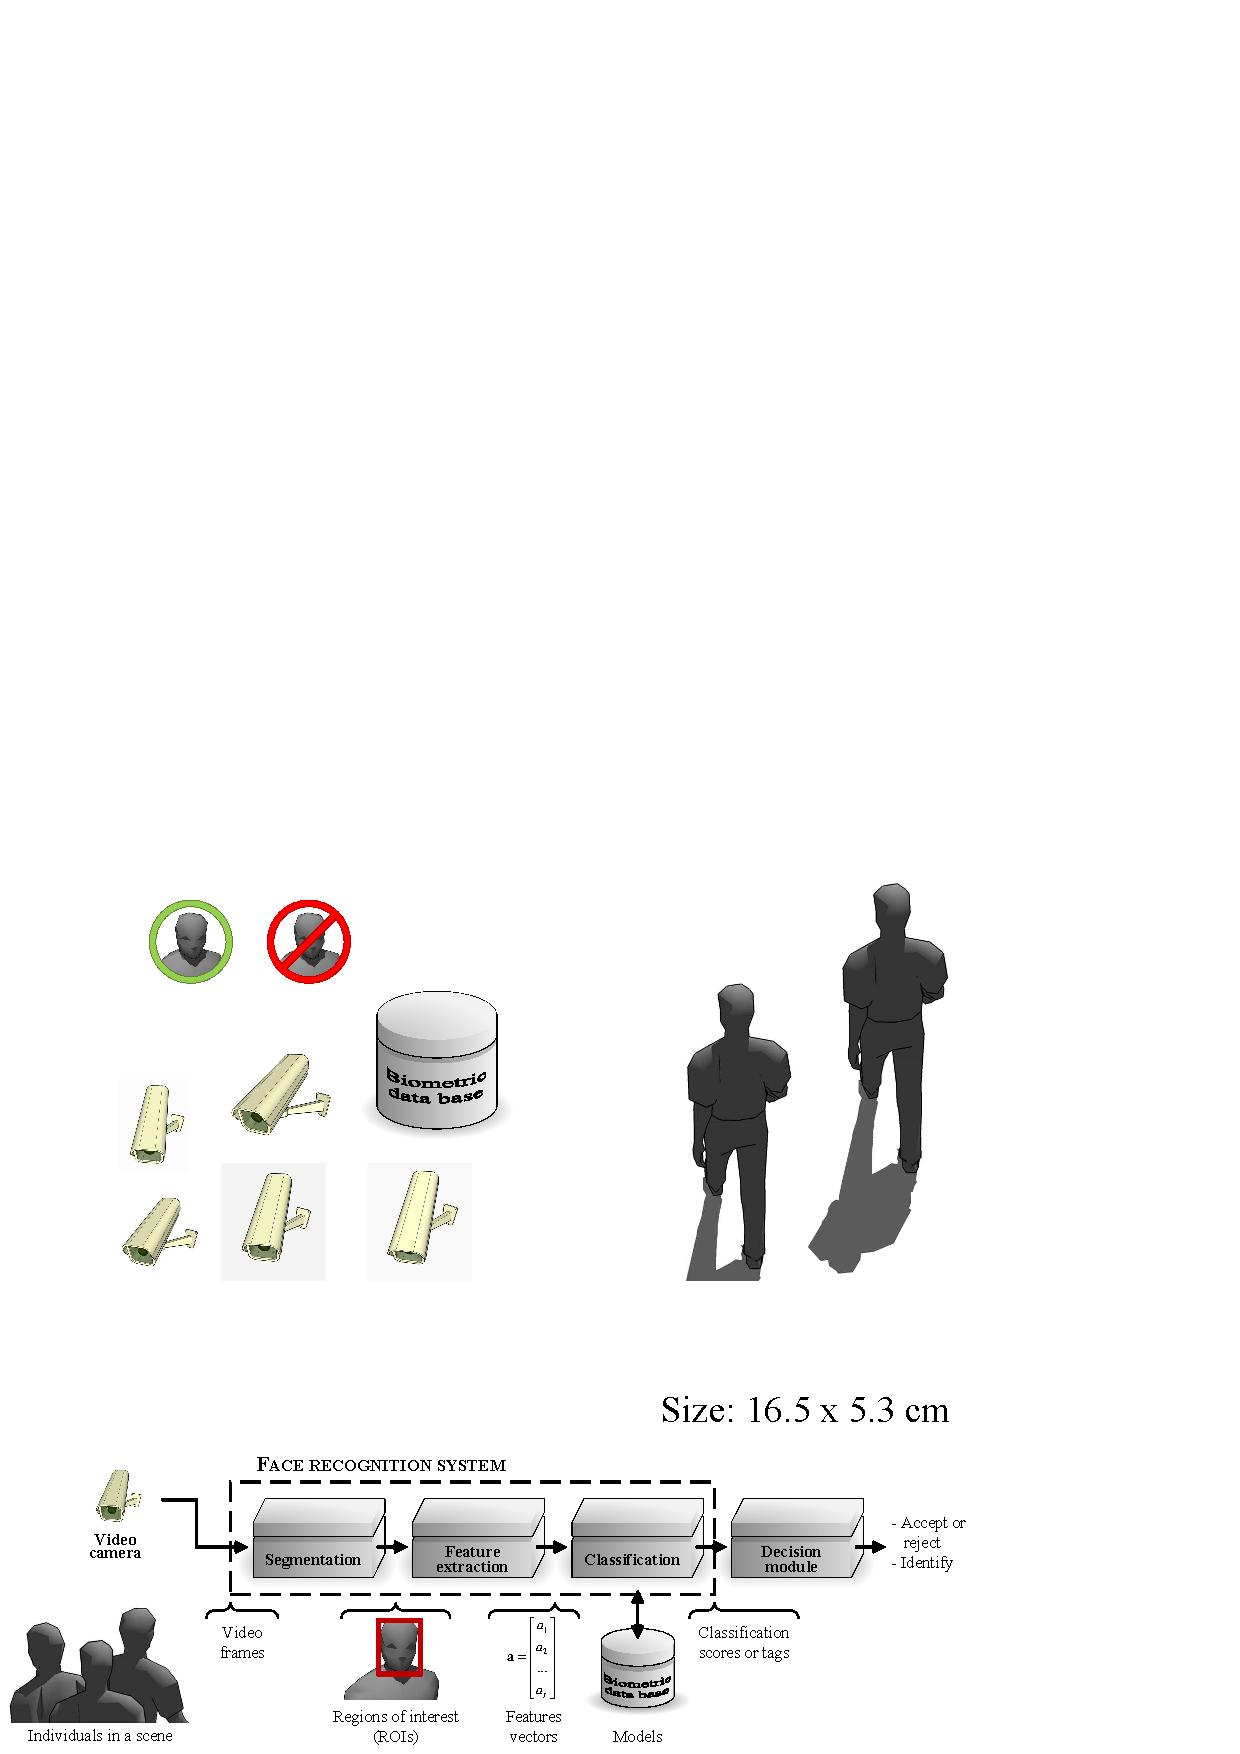
\includegraphics[width=0.97\linewidth, viewport= 0cm 0cm 16.5cm 5.3cm, clip]
 		              {c1_fig1}	}
  \caption{A general biometric system for face recognition. In this chapter, both classification module and biometric data base are replaced by the adaptive classification system}
	\label{fig:c1_faceRec}
\end{figure*}
%-------------------------- /Face recogniton system ---------------------------%

More recently, some authors have combined spatial and temporal information contained in video sequences to provide a higher level of accuracy in unconstrained scenes (\cite{matta09}). These track-and-classify systems combine the responses of a classifier to kinematic information of individuals and faces in a scene. For instance, a distributed sensor network is proposed by \cite{foresti02} as a solution to the problem of partial occlusion that occurs in dynamics environments. \cite{li01} have introduced a face verification system which exploits the trajectories of Gabor facial features to identify individuals through hypothesis testing, using a posterior density characterized by the motion. A time series states space has been proposed by \cite{zhou03} to fuse temporal information in video, which simultaneously characterizes the kinematics and identity of individuals in a probabilistic framework. \cite{barry07} have applied the What-and-Where Fusion neural network to the identification of individuals. This network simultaneously tracks multiple faces in an environment and accumulates their classifier predictions over time to improve classification. \cite{matta07} uses a multimodal system integrating the displacement signals of the head and physiological information with a probabilistic extension of the Eigenface approach. \cite{majumdar08} proposed an image-to-image-based recognition approach that uses color information and a kernel classifier for face authentication. Finally, \cite{mian08} uses an unsupervised learning approach to determine the identity of an individual on the basis of best temporally cohesive matches between clusters of video sequence.

With these systems, the underlying data distribution $p(\textbf{a})$ is considered static in nature and learning occurs only once, during a preliminary design phase. As discussed, once the face recognition system is deployed, temporary and permanent changes may occur in complex real-world environments and the initial learning data may no longer be representative nor sufficient to properly define the underlying class probability distributions $p_k(\textbf{a})$. This may lead to significant degradation in performance during operations. Assuming that new data becomes available, classifiers found in most face recognitions systems in literature would require relearning from the start using all previously acquired data through supervised batch learning. Performing incremental learning with only the new data would therefore be an undisputed asset as the memory and time complexity associated with storing and training is greatly reduced. In addition, it can maintain a high level of performance by reducing the divergence between class models and underlying distributions.

%--------------------------------- Adaptation ---------------------------------%
\section{Adaptive classification system}
\label{sec:c1_adaptation}

Figure \ref{fig:c1_framework} depicts the evolution of the adaptive classification system (ACS) proposed in this chapter for supervised incremental learning of new data. This novel system is composed of a pattern classifier that is suitable for supervised incremental learning, a dynamic optimization module that tunes the user-defined hyperparameters of the classifier, and a long term memory (LTM) that manages and stores incoming learning data used for validation and fitness evaluation.

When a new block of learning data $D_t$ becomes available to the system at a discrete time $t$, part of the data is employed to train the incremental classifier and update the LTM. The classifier then interacts with the dynamic optimization module using a DPSO-based algorithm that cojointly optimizes the vector of user-defined hyperparameters $\textbf{h}$, parameters, and architecture such that classification rate maximized. In this chapter, the fuzzy ARTMAP neural network (\cite{carpenter92}) is employed as an incremental learning classifier and a dynamic version the particle swarm optimization (PSO) algorithm (\cite{kennedy95}) is used for optimization.


%------------------------- Framework - for section 2 --------------------------%
\begin{figure*}[t]
  \centering
	\fbox{
  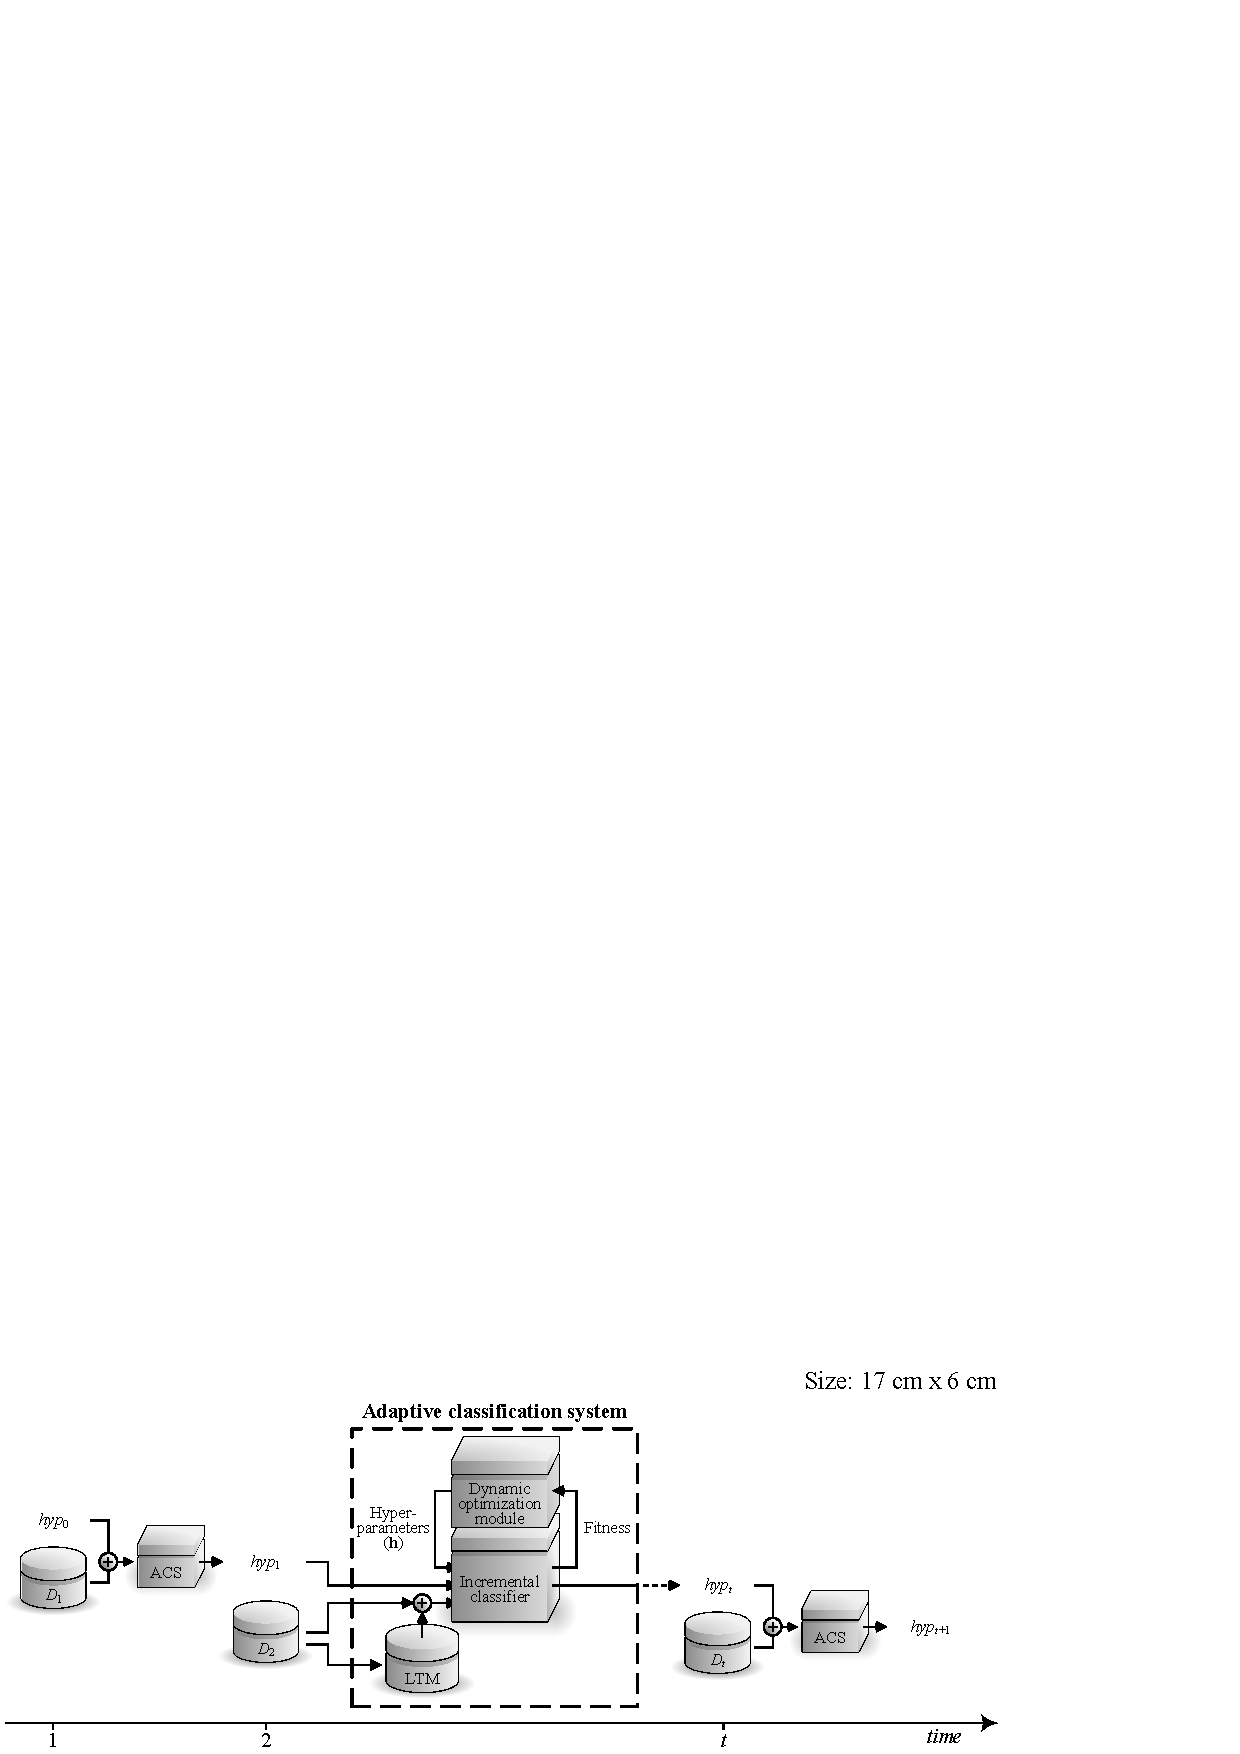
\includegraphics[width=0.97\linewidth, viewport =0cm 0cm 17cm 6cm, clip]
  								{c1_fig2} }
  \caption{The evolution of a new adaptive classification system (ACS) according to generic incremental learning scenario. New blocks of data are used by the ACS to update the classifier over time. Let $D_1$, $D_2$, … be blocks of learning data available at different instants in time. The ACS starts with an initial hypothesis $hyp_0$ which constitutes the prior knowledge of the domain. Each hypothesis $hyp_{t-1}$ are updated to $hyp_t$ by the ACS on the basis of the new data block $D_t$}
	\label{fig:c1_framework}
\end{figure*}
%------------------------------------------------------------------------------%

Most techniques used to optimize fuzzy ARTMAP hyperparameters found in literature allow the optimization of only one or two hyperparameters, even though there are four inter-dependent parameters (\cite{canuto00, dubrawski97, fung03}). In previous work, the authors have introduced a PSO-based learning strategy for mono-objective optimization of all four hyperparameters (\cite{granger07}). It is based on the concept of neural network evolution in that it determines the optimal vector hyperparameters and network weights and architecture such that classification rate is maximized. The PSO strategy has been shown to provide a significantly higher classification rate on several synthetic and real-world data sets (\cite{barry07, granger07}).

While a key feature of ARTMAP networks is their ability to learn new information incrementally, without catastrophic forgetting, those optimization methods have all been developed for batch supervised learning of a finite data set The adjustment of fuzzy ARTMAP hyperparameter vector\footnote{Let $\textbf{h}$ be a vector of user-defined hyperparameters that set classifier dynamics. For fuzzy ARTMAP, it is composed of the four hyperparameters $\textbf{h}=(\alpha, \beta, \epsilon, \bar{\rho})$ described in Section \ref{sec:c1_fam}.} $\textbf{h}$ is then defined as the static optimization problem such that:
\begin{equation}
	\textnormal{maximize }\left\{ f(\textbf{h})\ |\ \textbf{h} \in \mathbb{R}^4 \right\},
	\label{eq:c1_optSta}
\end{equation}
where the objective function $f(\textbf{h})$ is the classification rate. In contrast, the ACS proposed in Figure \ref{fig:c1_framework} performs incremental learning. As shown in Appendix \ref{sec:c1_2Dresult}, incremental learning of new data from the class probability distributions $p_k(\textbf{a},t)$ translates to an objective function $f(\textbf{h})$ that also changes in time. Adapting fuzzy ARTMAP hyperparameters vector \textbf{h} during incremental learning of data blocks $D_t$ to maximize classification rate can thus be formulated as a dynamic optimization problem such as:
\begin{equation}
	\textnormal{maximize }\left\{ f(\textbf{h},t)\ |\ \textbf{h}\in\mathbb{R}^4,
															 t\in\mathbb{N}_1, \right\}
	\label{eq:c1_optDyn}
\end{equation}
where $f(\textbf{h},t)$ is the classification rate of fuzzy ARTMAP for a given vector of hyperparameters h, after learning data set $D_t$ and at a discreet time $t$.

For an optimization space defined by fuzzy ARTMAP hyperparameters, three different types of dynamic optimization environment are then possible (\cite{engelbrecht05}):
\begin{itemize}
	\item \emph{type I environments} where the location of the optimum changes over time,
	\item \emph{type II environments} where the location of the optimum remains fixed, but the value of the objective function at the position of the optimum changes, and
	\item \emph{Type III environments} where both the location and the value of
				optima points change.
\end{itemize}
As results presented in Appendix \ref{sec:c1_2Dresult} suggest the presence of a type III optimization environment for fuzzy ARTMAP hyperparameters adjustment during incremental learning. The ACS employs a DPSO algorithm called Dynamic Niching PSO designed for such environments (\cite{nickabadi08_2}). The rest of this section provides additional details on each part of the adaptive classification system: the long term memory, the fuzzy ARTMAP neural network, and the DPSO-based learning strategy.

%------------------------ Subsection : Long term memory -----------------------%
\subsection{Long term memory}
\label{sec:c1_LTM}

During incremental learning, each new learning block of data $D_t$ is divided into $D_t^\text{t}$ and $D_t^\text{v}$ for training with validation over several training epochs,\footnote{An epoch is defined as one complete presentation of all the patterns of a finite training data set.} and into $D_t^\text{f}$ for estimation of the fitness on the objective function $f(\textbf{h},t)$.

%------------------------------ Data organization -----------------------------%
\begin{figure*}[t]
  \centering
	\fbox{
 	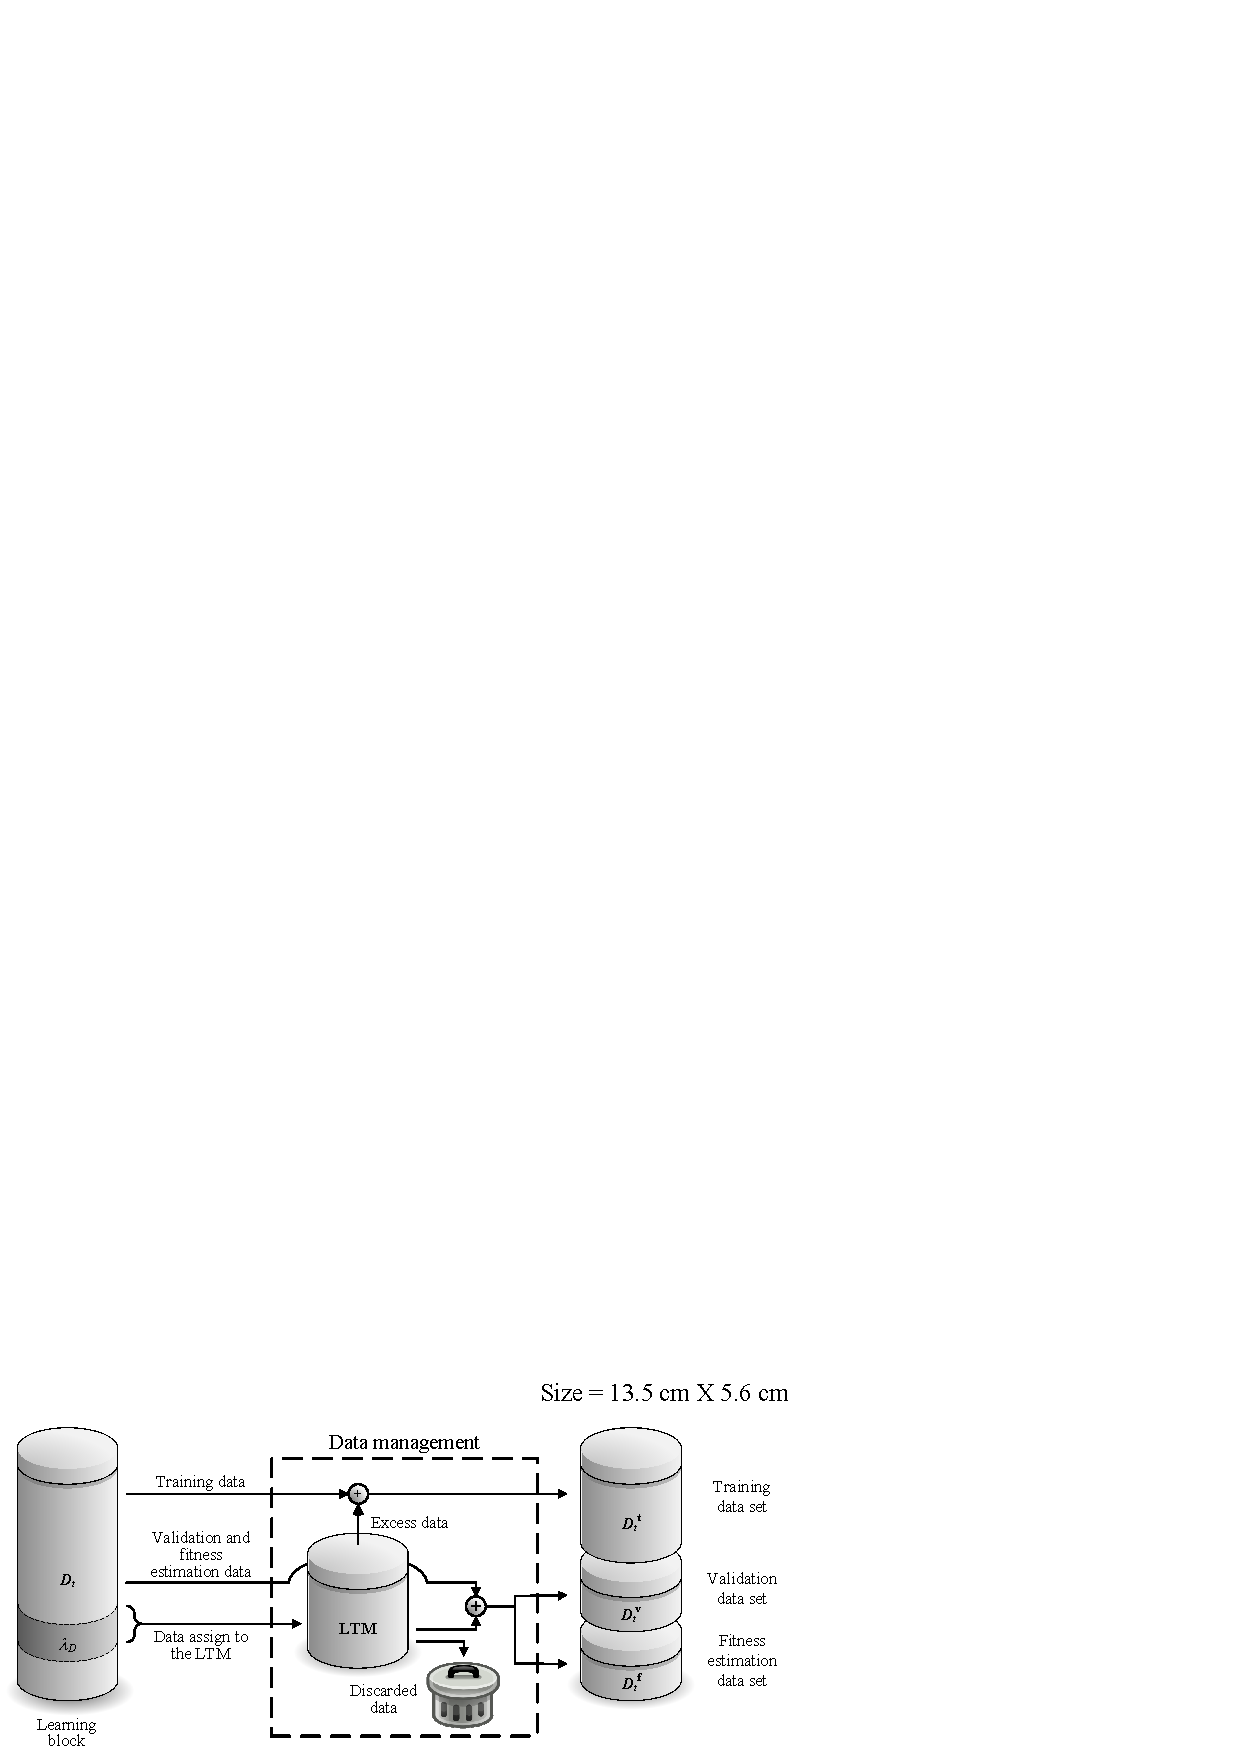
\includegraphics[width=0.97\linewidth, viewport= 0cm 0cm 13.5cm 5.6cm, clip]
								  {c1_fig3}
	}
  \caption{Data management for the learning process using the long term memory. When a learning block $D_t$ is available, a proportion $\lambda_D$ of this data is assigned to the long term memory, and the rest is used for training, validation, and performance estimation. When the LTM is updated, old data is discarded, while excess data not used to fill and/or update the LTM (dues to size limitations) is integrated to the training data from $D_t$ to create the training data set $D_t^\text{t}$. Data contained in the LTM is then combined with data coming directly from $D_t$ dedicated to validation and fitness estimation. This combination is class-wise divided in two, to create the validation data set $D_t^\text{v}$ and the fitness estimation data set $D_t^\text{f}$}
 	\label{fig:c1_LTM}
\end{figure*}
%----------------------------- /Data organization -----------------------------%

It has been shown in \cite{connolly09}, that the data sets used to guide the particles in the optimization space during a PSO-based incremental learning algorithm ($D_t^\text{f}$) should contain a representative set of samples from all classes $C_k \in \Omega$ to avoid a decline in fuzzy ARTMAP performance. As Figure \ref{fig:c1_LTM} depicts, some of the data of each learning block is used to create and maintain a long term memory (LTM). The LTM functions according to two parameters: (1) the proportion of $D_t$ used to fill and update the external data base, $\lambda_D$, and (2) the maximal number of patterns per class in the external data base $|C_k|_\mathbf{LTM}$. Each time a new $D_t$ is presented to the network a proportion $\lambda_D$ of $D_t$ is randomly selected and transferred to the LTM for either addition or update. The LTM is managed as a FIFO (first in, first out) data structure, and the outdated data that surpasses $|C_k|_\mathbf{LTM}$ is discarded. For each class, if the number of patterns transferred exceeds $|C_k|_\mathbf{LTM}$, the excess samples are randomly selected and integrated to $D_t^\text{t}$.

%------------------------- Subsection : fuzzy ARTMAP --------------------------%
\subsection{Fuzzy ARTMAP Neural Networks}
\label{sec:c1_fam}

ARTMAP refers to a family of self-organizing neural network architectures that is capable of fast, stable, on-line, unsupervised or supervised, incremental learning, classification, and prediction (\cite{carpenter91}). A key feature of ARTMAP networks is their unique solution to the stability-plasticity dilemma. They can adjusts previously learned categories in response to familiar inputs, and creates new categories dynamically in response to inputs different enough from those previously seen.

Several ARTMAP networks have been proposed in order to improve the performance of these architectures. They can be broadly divided according to their internal matching process, which depends on either deterministic or probabilistic category activation. The deterministic type consists of networks such as fuzzy ARTMAP, ART-EMAP, ARTMAP-IC, default ARTMAP, simplified ARTMAP, distributed ARTMAP, etc., and represent each class using one or more category hyper-rectangles. In contrast, the probabilistic type consists of networks such as PROBART, PFAM, MLANS, Gaussian ARTMAP, ellipsoid ARTMAP, boosted ARTMAP, $\mu$ARTMAP, etc., and represent each class using one or more probability density functions.

The fuzzy ARTMAP integrates the fuzzy ART to process both analog and binary-valued input patterns to the original ARTMAP architecture (\cite{carpenter92}). This simple and popular neural network has been designed with the ability to perform supervised incremental learning as defined in \cite{polikar01}. In supervised learning mode, the sequential learning process grows the number of recognition categories according to a problem's complexity. The vigilance and match tracking process provide the mechanisms to control the local impact of new data on the existing knowledge structure. Even if fuzzy ARTMAP is able to perform well with few training data (\cite{hennegis06}), previous research by the authors has revealed that the average classification rate of an ARTMAP network trained through incremental learning is usually significantly lower than if trained on all the data through batch learning (\cite{granger08, connolly08}).

%-------------------------------- Fuzzy ARTMAP --------------------------------%
\begin{figure}[!t]
  \centering
	\fbox{
  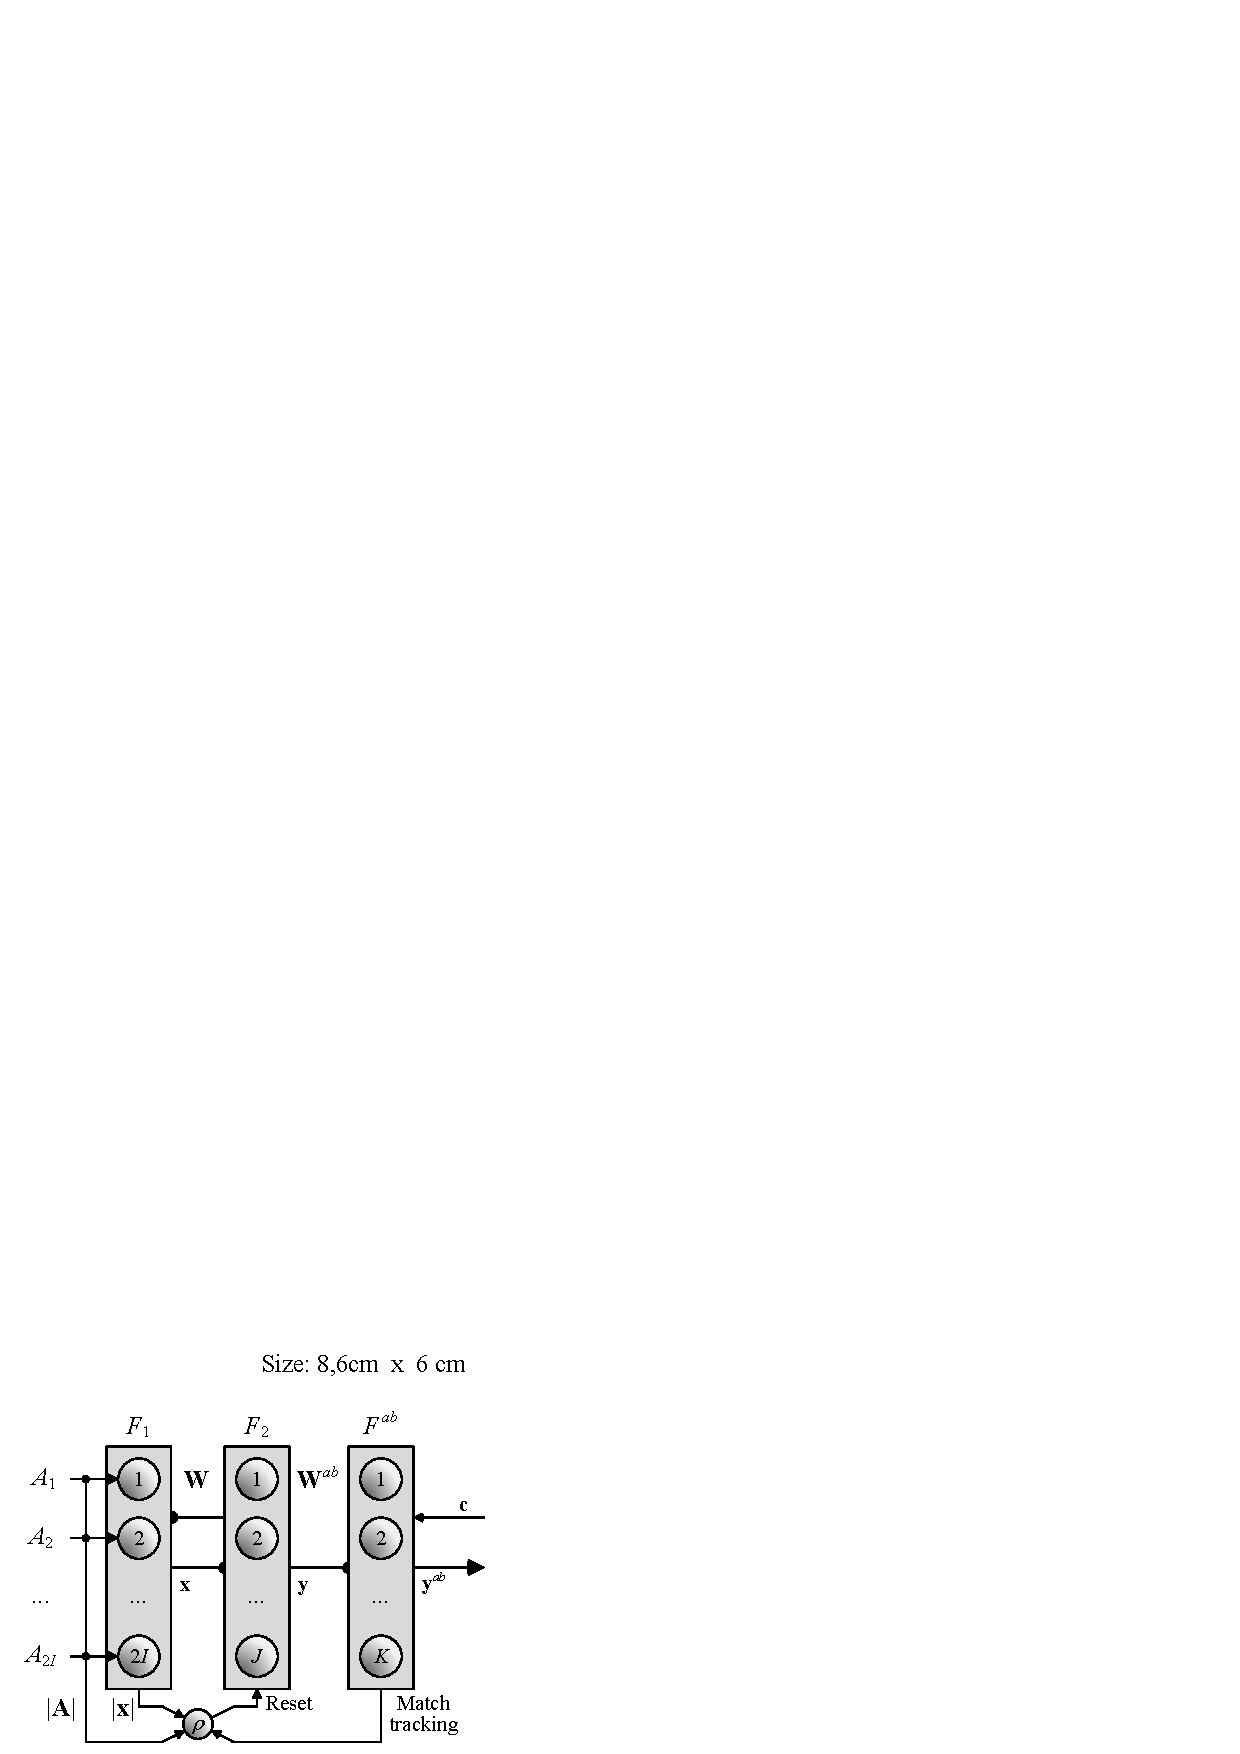
\includegraphics[width=0.5\linewidth, viewport=0cm 0cm 8.6cm 6cm, clip]{c1_fig4}
	}
  \caption{Fuzzy ARTMAP neural network}
	\label{fig:c1_fam}
\end{figure}
%------------------------------------------------------------------------------%

Fuzzy ARTMAP consists of three layers (Figure \ref{fig:c1_fam}): (1) an input layer $F_1$ of $2I$ neurons (for a $\mathbb{R}^I$ input feature space), (2) a competitive layer $F_2$ of $J$ neurons, and (3) a map field $F^{ab}$ of $K$ neurons (the number of classes). The $F_1$ and $F_2$ layers are connected through a set of real-valued weights $\textbf{W} = \{w_{ij} \in [0,1] : i = 1, 2, ..., 2I; j = 1, 2, ..., J\}$ and the $F_2$ layer is connected, through learned associative binary weights $\textbf{W}^{ab} = \{w^{ab}_{jk} \in \{0,1\} : j = 1, 2, ..., J;\, k = 1, 2, ..., K\}$, to a $K$ nodes map field $F^{ab}$. Each $F_2$ node $j$ represents a recognition category as an $I$-dimensional hyper-rectangle in the feature space, and is associated to one of the K output classes with the vector $\textbf{w}^{ab}_j = (w^{ab}_{j1}, w^{ab}_{j2}, ..., w^{ab}_{jK})$. The weights connected to each node correspond to a prototype vector $\textbf{w}_j = (w_{1j}, w_{2j},..., w_{2Ij})$.

In supervised training mode, ARTMAP classifiers learn an arbitrary mapping between training set patterns $\textbf{a}$ = $(a_1, a_2, ..., a_I)$ and their corresponding binary supervision patterns $\textbf{c}$ = $(c_1, c_2, ..., c_K)$.
These patterns are coded to have unit value $c_k = 1$ if $k$ is the target class
label for $\textbf{a}$, and zero elsewhere. The following algorithm describes fuzzy ARTMAP learning:
\begin{enumerate}
    \item \emph{Initialization:} Initially, all the $F_2$ nodes are uncommitted, all weight values wij are initialized to 1, and all weight values  are set to 0. An $F_2$ node becomes committed when it is selected to code an input vector $\textbf{a}$, and is then linked to an $F^{ab}$ node. Values of the learning $\beta \in [0,1]$, choice $\alpha>0$, match tracking $\epsilon=0^+$, and baseline vigilance $\bar{\rho} \in [0,1]$ parameters are set.
    \label{step:initialization}

		\item \emph{Input pattern coding:} When a training pair $(\textbf{a}, \textbf{c})$ is presented to the network, a undergoes a transformation called complement coding, which doubles its number of components. The complement-coded input pattern has $2I$ dimensions and is defined by $\textbf{A}$ = $(\textbf{a},\textbf{a}^{c})$ = $(a_1, a_2, ..., a_I; a^c_1, a^c_2, ..., a^c_I)$, where $a^c_i = (1-a_i)$, and $a_i \in [0,1]$. The vigilance parameter $\rho$ is reset to its baseline value $\bar{\rho}$.
		\label{step:coding}

		\item \emph{Prototype selection:} Complement-coded pattern $\textbf{A}$ activates layer $F_1$ and is propagated through weighted connections $\textbf{W}$ to layer $F_2$. Activation of each node $j$ in the $F_2$ layer is determined by the \emph{Weber law choice function}:
		\begin{equation}
			\label{eq:c1_choice}
			T_j(\textbf{a}) = \frac{ |\textbf{A} \wedge \textbf{w}_j| }
														{ \alpha + |\textbf{w}_j|          } \ ,
		\end{equation}
		where $|\ \cdot\ |$ is the $L^1$ norm operator defined by $|\textbf{w}_j| 
		\equiv \sum_{i=1}^{2I} |w_{ij}|$, $\wedge$ is the fuzzy AND operator,
		$(\textbf{A} \wedge \textbf{w}_j)_i \equiv \min(A_i,w_{ij})$, and $\alpha$ is the user-defined \emph{choice parameter}.
		The $F_2$ layer produces a binary, winner-take-all pattern of activity $\textbf{y} = (y_1, y_2, ..., y_J)$ such that only the node $j = j^*$ with
		the greatest activation value $j^* = \arg \max \{T_j : j = 1, 2, ..., J\}$ remains active; thus $y_{j^*} = 1$ and $y_j = 0, j \neq j^*$. If more than one $T_j$ is maximal, the node $j$ with the smallest index is chosen.
		Node $j^*$ propagates its top-down expectation, or prototype vector $\textbf{w}_{j^*}$, back onto $F_1$ and the \emph{vigilance test} is performed.
		This test compares the degree of match between $\textbf{w}_{j^*}$ and
		$\textbf{A}$ against the dimensionless \emph{vigilance parameter} $\rho
		\in [0,1]$:
		\begin{equation}\label{eq:c1_vigilance}
				\frac{|\textbf{A} \wedge \textbf{w}_{j^*}|}{|\textbf{A}|} =
				\frac{|\textbf{A} \wedge \textbf{w}_{j^*}|}{I} \geq \rho \ .
		\end{equation}
		If the test is passed, then node $j^*$ remains active and resonance is said
		to occur. Otherwise, the network inhibits the active $F_2$ node ({\em \emph{i.e.},}
		$T_{j^*}$ is set to 0) until Step \ref{step:selection} begins anew, and
		continues searching for another node $j^*$ that passes the vigilance test.
		If such a node does not exist, an uncommitted $F_2$ node becomes active and undergoes learning (Step~\ref{step:learning}).
		\label{step:selection}

		\item \textbf{Class prediction:} Pattern $\textbf{c}$ is fed directly to the map field $F^{ab}$, while the $F_2$ category $\textbf{y}$ learns to activate the map field via associative weights $\textbf{W}^{ab}$. The $F^{ab}$ layer produces a binary pattern of activity $\textbf{y}^{ab}	= (y^{ab}_1, y^{ab}_2, ..., y^{ab}_K) = \textbf{t} \wedge \textbf{w}^{ab}_{j^*}$ in which the most active $F^{ab}$ node $k^* = \arg\max \{y^{ab}_k : k = 1, 2, ..., K\}$ yields the class	prediction ($k^*=k(j^*)$). If node $k^*$ constitutes an incorrect class prediction, then a \emph{match tracking} signal adjust the vigilance parameter $\rho$ according to:
		\begin{equation}\label{eq:c1_mt}
			\rho = \frac{|\textbf{A} \wedge \textbf{w}_{j^*}|}{I} + \epsilon \ ,
		\end{equation}
the network deactivates node $j^*$ until the network is presented with the next training pair $(\textbf{a}, \textbf{c})$), and another search is induced among $F_2$ nodes in Step \ref{step:selection}. This search continues until either an uncommitted $F_2$ node becomes active (and learning directly ensues in Step~\ref{step:learning}), or a node $j^*$ that has previously learned the correct class prediction $k^*$ becomes active.
		\label{step:prediction}

    \item \textbf{Learning:} Learning input $\textbf{a}$ involves updating prototype vector $\textbf{w}_{j^*}$, and, if $j^*$ corresponds to a newly-committed node, creating an associative link to $F^{ab}$. The prototype vector of $F_2$ node $j^*$ is updated according to:
        \begin{equation}\label{eq:c1_learning}
            \textbf{w}_{j^*}' = \beta\ (\textbf{A} \wedge \textbf{w}_{j^*}) + 
            									  (1 - \beta) \textbf{w}_{j^*} \ ,
        \end{equation}
where $\beta$ is a fixed \emph{learning rate parameter}. A new association between $F_2$ node $j^*$ and $F^{ab}$ node $k^*$ ($k^* = k(J)$) is learned by setting $w^{ab}_{j^*k}=1$ for $k=k^*$, where $k^*$ is the target class label for $\textbf{a}$, and 0 otherwise.
      The next training subset pair $(\textbf{a}, \textbf{c})$ is presented to
      the network in Step \ref{step:coding}.
    \label{step:learning}
\end{enumerate}
Once the weights $\textbf{W}$ have been found through this process, ARTMAP can predict a class label for an input pattern by performing Steps \ref{step:coding}, 3 and 4 without any vigilance or match tests. During testing, a pattern $\textbf{a}$ that activates node $j^*$ is predicted to belong to class $k^*=k(j^*)$.

During training and testing fuzzy ARTMAP internal dynamic is governed by four user-defined hyperparameters: the choice parameter $\alpha$, the learning parameter $\beta$, the match tracking parameter $\epsilon$, and the baseline vigilance parameter $\bar{\rho}$. Each of these hyperparameters are inter-related, and has a distinct impact on network dynamics. While $\alpha$ and $\epsilon$ determine the depth of search attained before an uncommitted node is selected in the learning algorithm during Steps \ref{step:selection} (Equation \ref{eq:c1_choice}) and \ref{step:prediction} (Equation \ref{eq:c1_mt}),  limits the maximum expansion of the recognition categories in the $\mathbb{R}^I$ feature space (Equation \ref{eq:c1_vigilance}). Low vigilance allows large hyper-rectangles and leads to broad generalization and abstract memories, while high vigilance yields small hyper-rectangles, leading to narrow generalization and detailed memories. During Step \ref{step:learning}, $\beta$ determines the speed with which the recognition categories are expanded to fit \textbf{a}. The algorithm can be set to slow learning with $0<\beta<1$, or to fast learning with $\beta = 1$. With fast learning, each hyper-rectangle is just large enough to enclose the cluster of training set patterns \textbf{a} to which it has been assigned. That is, an $I$-dimensional prototype vector $\textbf{w}_j$ records the largest and smallest component values of training subset patterns \textbf{a} assigned to category $j$. A standard vector of hyperparameters $\textbf{h}_\text{std} = \left(\alpha = 0.001, \beta=1,\epsilon=0.001,\bar{\rho}=0\right)$ is commonly used to minimize network complexity (\cite{carpenter92}).

%------------------------------ subsection : pso ------------------------------%
\subsection{Dynamic particle swarm optimization}
\label{sec:c1_dpso}

Particle swarm optimization (PSO) is a population-based stochastic optimization technique that was inspired by social behavior of bird flocking or fish schooling (\cite{kennedy95, kennedy07}). With PSO, each particle corresponds to a single solution in the optimization space, and the population of particles is called a swarm. Particles move through the optimization space and change their course under the guidance of a cognitive influence (\emph{i.e.}, their own previous search experience) and a social influence (\emph{i.e.}, their neighborhood previous search experience) and unlike evolutionary algorithms (such as genetic algorithms), each particle always keep in memory its best position and the best position of its surrounding.

Originally developed for static optimization problems, the PSO algorithm has been adapted for dynamic optimization problems by adding mechanisms to (1) modify the social influence to maintain diversity in the optimization space and detect several optima, (2) detect changes in the objective function by using the memory of each particle, and (3) adapt the memory of its population if change occur in the optimization environment. The latest PSO algorithms developed to insure diversity in the swarm are presented in \cite{du08, li06, nickabadi08_1, ozcan07}, while change detection and memory adjustment mechanisms are presented in \cite{blackwell04, carlisle02, hu02, wang07}.

When the ACS learns a new data blocks $D_t$ (Figure \ref{fig:c1_framework}), a Dynamical Niching PSO (DNPSO) algorithm adapted for dynamic optimization (\cite{nickabadi08_2}) is used to maximize fuzzy ARTMAP classification rate as function of its hyperparameters vector $\textbf{h}=\left(\alpha, \beta, \epsilon, \bar{\rho}\right)$. The optimization space is defined by the four fuzzy ARTMAP hyperparameters, and the performance of each particle's position is its value on the objective function $f(\textbf{h},t)$.

This PSO algorithm is simple to implement and has been shown to rapidly converge toward global maximum in a multimodal type III optimization environment with the moving peaks benchmark (\cite{nickabadi08_2}). It maintains diversity with a local neighborhood topology and by dynamically creating subswarms around certain particles, called masters, that are their own best position amongst their neighborhood. Particles that are not part of any subswarms are called free particles and are allowed to move by themselves. Once the subswarms have been defined, position of particles that are members of a subswarm are updated using
\begin{equation}
	\begin{split}
		\textbf{h}_n(\tau+1) = & \ \textbf{h}_n(\tau) 
                    + w_0\ ( \textbf{h}_n(\tau) - \textbf{h}_n(\tau-1) )\\
	  							& + r_1\ w_1/2\ 
                      ( \textbf{h}^*_{\textit{master}} - \textbf{h}_n(\tau) )\\
     							& + r_2\ w_1/2\ 
                      ( \textbf{h}^*_n -                 \textbf{h}_n(\tau) ),  	
	\end{split}
	\label{eq:c1_psoSs}
\end{equation}
where $\textbf{h}_n(\tau)$ is the position of particle $n$ in the optimization space at iteration $w_0$ and $w_1$ are inertia weights, $r_1$ and $r_2$ are random numbers generated at each iteration, $\textbf{h}_n(\tau)$ and $\textbf{h}^*_n$ are respectively the current position of the subswarm master's personal best (social influence) and particle $n$ personal best (cognitive influence). On the other hand, free particles move only according to their own cognitive influence using:
\begin{equation}
	\begin{split}
		\textbf{h}_n\left(\tau+1\right) = & \ \textbf{h}_n(\tau) 
                      + w_0\ ( \textbf{h}_n(\tau) - \textbf{h}_n(\tau-1) )\\
										& + r_3\ w_1\ ( \textbf{h}^*_n - \textbf{h}(\tau) ), 
  \end{split}
	\label{eq:c1_psoF}
\end{equation}
where $r_3$ is another random number generated at each iteration. The global best particle is referred to as $gbest$, and in case there is a tie for the global best position, the particle with the smallest index wins. If the maximal number of subswarms is set to one, its maximal size and the neighborhood size is equal to the swarm's total number of particles, the DNPSO is then equivalent to the canonical PSO described in \cite{kennedy95}. All the particles will then converge toward the only master (\emph{i.e.}, the global best) according to Equation \ref{eq:c1_psoSs}.

Initially developed in \cite{nickabadi08_1}, DNPSO was adapted for dynamic optimization problem by simply updating the performance of their best position $f(\textbf{h}^*_n,t)$ at each iteration. Normally, for DPSO algorithms, this would double the number of time values on the objective function are evaluated, leading to a very costly process. For our ACS, changes in the objective function only occur only when a new data block $D_t$ becomes available. Thus, the performance of the particles best position is only updated when $D_t$ is presented to the system, \emph{before} the iterative DNPSO process.

Algorithm \ref{alg:c1_pso} describes the DPSO-based incremental learning strategy for co-optimization of hyperparameters, weight and architecture of the fuzzy ARTMAP neural network. Given new learning data block $D_t$, it produces the optimal set of hyperparameters and network using a particle swarm with $N$ particles, and $N+2$ fuzzy ARTMAP neural networks -- one network per particle $\textit{FAM}_n$, used to preserve the model associated to the best position of that particle ($\textbf{h}^*_n$), one temporary neural network used for the fitness estimation during the algorithm ($\textit{FAM}_\text{estimation}$), and one optimal network ($\textit{FAM}_\text{optimal}$).

%------------------------------ Algorithm : pso -------------------------------%
\begin{algorithm}[t]
	\caption{DPSO-based incremental learning strategy for the ACS using a fuzzy ARTMAP neural network classifier}
	\label{alg:c1_pso}
 	\fbox{\begin{minipage}{0.97\linewidth}\centering
	\begin{algorithmic}[1]
		\Require A particle swarm with DNPSO parameters,
						 neural networks: $\textit{FAM}_{n}$, where $1\leq n\leq N$,
						 $\textit{FAM}_\text{estimation}$, and $\textit{FAM}_\text{optimal}$,
						 and new data sets $D_t$ for learning.
		\Ensure (1) $\textit{FAM}_\text{optimal}$ (Weights and architecture obtained
						with the optimal $\textbf{h}$) and  (2) $\textit{FAM}_n$ where $ 1
						\leq n \leq N$ (Set of fuzzy ARTMAP neural networks associated to 
						the best position of each particles).

		\Statex\vspace{6pt}\textbf{Initialization:}\vspace{3pt}
		
		\State Set the swarm parameters ($N$, $w_0$, $w_1$).   \label{l:c1_setSwarm}
		\State Randomly initialize particles positions for $t=0$
					 and $t=-1$ within their range.									\label{l:c1_swarmInit}
		\State Initialize $\textit{FAM}_\text{optimal}$ and all
					 $\textit{FAM}_{n}$, where $1\leq n\leq N$.			  \label{l:c1_initNN}
		\State Set PSO iteration counter at $\tau=0$.           \label{l:c1_itinit}
					 
		%-- For each learning block
		\Statex\vspace{9pt}\textbf{Upon reception of a new data block $D_t$, the
					 following incremental process is initiated:}\vspace{6pt}
		%-- Personnal best update
		\Statex\textit{Update the fitness of networks associated to the 
					  personal best positions:}\vspace{3pt}
		\For{ each particle $n$, where $ 1 \leq n \leq N$ }
			\State $\textit{FAM}_n \leftarrow \textit{FAM}_\text{optimal}$
																						          \label{l:c1_curUpdate}
			\State Training of $\textit{FAM}_n$ with validation using
						 $D_t^\text{t}$ and $D_t^\text{v}$, and  $f(\textbf{h}^*_n, t)$	
						 estimation using $D_t^\text{f}$.         \label{l:c1_trnUpdate}				\EndFor
		
		%-- Loop iterations
		\Statex\vspace{6pt}\textit{Optimization process:}\vspace{6pt}
		\While{ DNPSO did not reach stopping condition }
			\State Define the subswarms and update position of 
						 each particle with equations
						 \ref{eq:c1_psoSs} and \ref{eq:c1_psoF}.	\label{l:c1_newPos}
				\For{each particle $n$, where $ 1 \leq n \leq N$}
					\State $\textit{FAM}_\text{estimation}$ $\leftarrow$ 		
								 $\textit{FAM}_\text{optimal}$              \label{l:c1_curInit}
					\State Training of $\textit{FAM}_\text{estimation}$ with validation using
								 $D_t^\text{t}$ and $D_t^\text{v}$, and \\ \hspace{36pt}
								 $f(\textbf{h}_n(\tau),t)$ estimation using $D_t^\text{f}$.		      \label{l:c1_trn} 
				\EndFor
				\If{ $f(\textbf{h}_n(\tau),t) > f(\textbf{h}^*_n,t)$ }
					\State $\textbf{h}^*_n$ $\leftarrow$ $\textbf{h}_n(\tau)$								  \label{l:c1_pAssign}
					\State $f(\textbf{h}^*_n,t)$ $\leftarrow$ $f(\textbf{h}_n(\tau),t)$			  \label{l:c1_pfAssign}
					\State $\textit{FAM}_n$ $\leftarrow$
								 $\textit{FAM}_\text{estimation}$					  \label{l:c1_nnpAssign}
				\EndIf 
				\State $\tau = \tau + 1$											\label{l:c1_itUpdate}
			\EndWhile \label{for_iterations}
			
			\Statex\vspace{6pt}\textit{Define the neural network with the highest
			       accuracy:}\vspace{3pt}
			\State $\textit{FAM}_\text{optimal}$ $\leftarrow$
						 $\textit{FAM}_\textit{gbest}$									\label{l:c1_assignOpt}
			\label{l:c1_optEv}
	\end{algorithmic}
	\end{minipage} }
\end{algorithm}
%------------------------------------------------------------------------------%

First, at Line \ref{l:c1_setSwarm}, the DPSO swarm's parameters are set according to the DNPSO algorithm. Each particle position is then randomly initialized within their allowed range (Line \ref{l:c1_swarmInit}). All the neural networks ($\textit{FAM}_n$, $\textit{FAM}_\text{estimation}$, and $\textit{FAM}_\text{optimal}$) are initialized as described in Step \ref{step:initialization} of the fuzzy ARTMAP learning algorithm (Line \ref{l:c1_initNN}). To comply with Eqs. \ref{eq:c1_psoSs} and \ref{eq:c1_psoF}, a position at $t=-1$ is set in order to have an initial velocity. When a new block $D_t$ becomes available, the optimization process continues where it stopped with $D_{t-1}$ and the DNPSO algorithm updates the swarm's memory (Lines \ref{l:c1_curUpdate}--\ref{l:c1_trnUpdate}).\footnote{Dynamic PSO algorithms usually involve change detection at this point, while for static optimization, no detection is done and the swarm's memory remains intact} The network $\textit{FAM}_\text{optimal}$ found with $D_{t-1}$ is then copied to each $\textit{FAM}_n$, and thus serves as the initial condition for learning of $D_t$. For the first learning block, $\textit{FAM}_\text{optimal}$ will be in an initial state.  $\textit{FAM}_n$ is then trained with validation using $D_t^\text{t}$ and $D_t^\text{v}$, its classification rate is estimated using $D_t^\text{f}$ and defined as the particle personal best fitness, $f(\textbf{h}_n^*,t)$. Since the fitness is defined by the classification rate obtained with $D_t^\text{f}$, if there is a tie for the personal best position, the particle $n$ with the smaller number of recognition categories is the personal best. The same procedure is also used to find the swarm's global best.

Unless the stopping criteria are reached (defined in Section \ref{sec:c1_methodology}), the DNPSO algorithm will iteratively evaluate each particle's fitness and update their position. The DNPSO algorithm first defines the subswarms and free particles, and computes the new particle positions using Eqs. \ref{eq:c1_psoSs} and \ref{eq:c1_psoF} (Line \ref{l:c1_newPos}). For each particle, the $\textit{FAM}_\text{optimal}$ found from $D_{t-1}$ is copied to $\textit{FAM}_\text{estimation}$ prior training (Line \ref{l:c1_curInit}). $\textit{FAM}_\text{estimation}$ is then trained using $D_t^\text{t}$ and $D_t^\text{v}$, and its fitness is estimated on the basis of $D_t^\text{f}$ (Line \ref{l:c1_trn}). Personal best position, fitness, and neural networks associated to the personal best $\textit{FAM}_n$ are then updated accordingly (Lines \ref{l:c1_pAssign}--\ref{l:c1_nnpAssign}). Once the optimization process is completed for $D_t$, the $\textit{FAM}_\textit{gbest}$ network, associated to the best vector of hyperparameters $\textbf{h}_\textit{gbest}$ is stored as $\textit{FAM}_\text{optimal}$ to preserve an optimal set of hyperparameters and network throughout the learning process (Line \ref{l:c1_assignOpt}).

To minimize the impact of pattern presentation order on fuzzy ARTMAP performance in the DPSO-based strategy, Lines \ref{l:c1_curUpdate}--\ref{l:c1_trnUpdate} and lines \ref{l:c1_curInit}--\ref{l:c1_trn} of Algorithm \ref{alg:c1_pso} are replaced with Algorithm \ref{alg:c1_5rep}. When a network $\textit{FAM}_\text{temp}$ is input, the classification rate is assessed on $D_t^\text{f}$ for fuzzy ARTMAP trained on  $D_t^\text{t}$ over five different random pattern presentation orders. Fitness estimation is defined by the mean classification rate of those five replications, and the neural network trained with the best pattern presentation order. For each random patterns presentation order of $D_t^\text{t}$, $\textit{FAM}_\text{optimal}$ is copied in $\textit{FAM}_\text{temp}$, $\textit{FAM}_\text{temp}$ is trained using $D_t^\text{t}$ and $D_t^\text{v}$, and classification rate over $D_t^\text{f}$ is evaluated. The $\textit{FAM}_\text{temp}$ network that provides the best classification rate is copied to $\textit{FAM}_\text{estimation}$, and $f(\textbf{h}(\tau),t)$ is defined as the mean classification rate over the five replications (Lines \ref{l:c1_mean}).

%----------------------------- Algorithm : 5 fold -----------------------------%
\begin{algorithm}[t]
	\caption{Evaluation of particle fitness for the DPSO incremental learning
					 strategy}
	\label{alg:c1_5rep}
 	\fbox{\begin{minipage}{0.97\linewidth}\centering
	\begin{algorithmic}[1]
		\Require Best temporary network, $\textit{FAM}_\textit{temp}$.
		\Ensure  A particle's performance and the best neural 
						 network to obtained that performance.
		\State Initialize $\textit{FAM}_\text{temp}$					\label{l:c1_initTemp}
		\For{5 patterns presentation order}
			\State $\textit{FAM}_\text{temp}
						 \leftarrow \textit{FAM}_\textit{optimal}$	\label{l:c1_initIntRep}
			\State Training of $\textit{FAM}_\text{temp}$ with
						 validation using $D_t^\text{t}$ and 
						 $D_t^\text{v}$, and evaluatuation of its 
						 classification rate using $D_t^\text{f}$		 \label{l:c1_trnV}
			\If{the classification rate is the best so far} 							 \label{l:c1_ifClass}
				\State $\textit{FAM}_\text{temp}$
							 $\leftarrow$ $\textit{FAM}_\text{estimation}$
			\EndIf \label{l:c1_endifClass}
		\EndFor
 		\State $\textit{FAM}_\text{estimation}$
 					 $\leftarrow$ $\textit{FAM}_\text{temp}$ 				 \label{l:c1_bestNN}
		\State $f(\textbf{h}_n(\tau),t)$ $\leftarrow$ mean classification
					 rate of the 5 replications 										 \label{l:c1_mean}
	\end{algorithmic}
	\end{minipage} }
\end{algorithm}
%------------------------------------------------------------------------------%

The computational time of Algorithm \ref{alg:c1_pso} at a time $t$ depends on the number of: training patterns , training epochs, $\textit{FAM}_n$ $F_2$ layer nodes ($J_n$), input features ($I$), DNPSO particles ($N$), DNPSO iterations before the optimization stopping conditions are met ($\tau^*$), and replications in Algorithm \ref{alg:c1_5rep}. Amongst those variables, $N$ and the number of replications during Algorithm \ref{alg:c1_5rep} are constant values, and the number of training epochs and $\tau*$ are limited to maximal values after which training and optimization are forced to stop. During incremental learning, the time complexity of the ACS is defined as the worst-case execution time required learn a new $D_t$. In the worse case scenario, the hyperparameters are set to build large neural networks such as $J_n = |D_1^\text{t}\cup ...\cup D_t^\text{t}|$ and complexity of Algorithm \ref{alg:c1_pso} is then $O(J_n \cdot |D_t^\text{t}| \cdot I)$.
During operation, the time complexity to process one input pattern is $O(J_n \cdot I)$. This is comparable to that of a fuzzy ARTMAP neural network alone.

The complexity of the DPSO strategy also depends on the time create subswarms and manage particle positions during DNPSO optimization process. However, in all cases, the complexity for the fitness evaluation of one particle is always greater than that of the DNPSO algorithm when it creates the subswarms and manages the particles in the optimization space. Thus, the complexity of the DNPSO algorithm itself should not be taken into consideration when using Algorithm \ref{alg:c1_pso}.

%------------------------------------------------------------------------------%
%---------------------- SECTION: Experimental methodology ---------------------%
\section{Experimental Methodology}
\label{sec:c1_methodology}

%---------------------------- SUBSECTION : Database ---------------------------%
\subsection{Video Data bases}
\label{sec:c1_db}

In order to observe the impact on system performance of supervised incremental learning, proof-of-concept simulations are performed with two real-world video data bases for face recognition. The first data base was collected by the Institute for Information Technology of the Canadian National Research Council (IIT-NRC) (\cite{gorodnichy05}). It is composed of 22 video sequences captured from 11 individuals positioned in front of a computer. For each individual, two color video sequences of about 15 s are captured at a rate of 20 frames/s with an Intel webcam of a $160\times120$ resolution that was mounted on a computer monitor. Of the two video sequences, one is dedicated to training and the other to testing. They are taken under approximately the same illumination conditions (no sunlight, only ceiling light evenly distributed over the room), the same setup, and almost the same background. For all persons in the data base, each face occupies between 1/4 to 1/8 of the image. This data base contains a variety of challenging operational conditions such as motion blur, out of focus factor, facial orientation, facial expression, occlusion, and low resolution.

Face detection is performed using the Viola-Jones algorithm included in the OpenCV C/C++ computer vision library (\cite{viola01}). It produced regions of interest (ROIs) between $29\times18$ and $132\times119$ pixels for each face detection in a video sequence. The number of ROIs detected per class for the IIT-NRC database is displayed in Table \ref{tab:c1_nrc}. The features presented to the classifier are independent of camera resolution and color since the ROIs are converted in grayscale and normalized to $24\times24$ images where the eyes are aligned horizontally, with a distance of 12 pixels between them. Each ROI is vectorized into $\textbf{a} = \{ a_1, a_2, ..., a_{576}\}$, where each feature $a_i \in [0,1]$ represents a normalized grayscale value.

%---------------------- NRC learning data set description ---------------------%
\begin{table*}[t]
	\footnotesize
  \centering
  \caption{Number of learning and test patterns per individual ($C_k\in\Omega$) for the IIT-NRC data base}
  \begin{tabular*}{\linewidth}{@{\extracolsep{\fill}}|l|llllllllllll|}
  	\hline
    {\bf Number} & \multicolumn{11}{|l|}{\bf Individuals} &
    \multirow{2}{*}{{\bf Total}}
    \\ %\cline{2-12}
    {\bf of ROIs}    & 1 & 2 & 3 & 4 & 5 & 6 & 7 & 8 & 9 & 10 & 11 &
    \\ \hline 
    Learning data & 140 &  39 & 160 & 130 & 175 & 128 
    				      & 180 &  97 & 178 & 160 & 140 & 1527
		\\ 
    Test data		  & 142 &  40 & 159 & 131 & 186 & 134 
    				      & 190 & 100 & 188 & 168 & 147 & 1585
		\\ \hline
	\end{tabular*}
	\label{tab:c1_nrc}
\end{table*}
%--------------------- /NRC learning data set description ---------------------%

The second video data base is the Motion of Body (MoBo), and was collected at Carnegie Mellon University under the HumanID project (\cite{gross02}). Each video sequences show one of 25 different individuals walking on a tread-mill so that they move their heads naturally to four different motion types when walking: slowly, fast, on an inclined surface, and while carrying an object. Six cameras are positioned at different locations around the individuals, and for each angle, individuals are filmed with a Sony DXC 9000 camera with a resolution of a $640\times480$ pixels.

The video sequences with visible faces (full frontal view and both sides with an angle of about $45^\circ$ with the full frontal view) where processed with the Viola-Jones algorithm for all four types of walk. This data base was reduced in order to use roughly the same size of the IIT-NCR data base, while having, for each individual, the same number of ROIs from each motion types and camera angle. Data from 10 individuals was employed, with 288 ROIs per class (24 ROIs for each type of walk and camera angle) for a total of 2880 patterns. The data base was divided into a learning and test data sets of 1440 patterns each. For each type of walk and camera angle, the first 12 of the 24 ROIs sequence were assign to the learning data set, while the last 12 were assign to the test data set. The ROIs were scaled and vectorized into $\textbf{a} = \{ a_1, a_2, ... , a_{576}\}$ as with the IIT-NRC data base.

%------------------------------------------------------------------------------%
\subsection{Incremental learning scenarios}
\label{sec:c1_scenario}

Prior to computer simulations, each video data set is divided in blocks of data $D_t$, where $1\leq t\leq T$, to emulate the availability of $T$ successive blocks of training data to the ACS. Supervised incremental learning is performed according two different scenario.

\subsubsection{Enrollment}

In this scenario, each block contains ROIs of individuals that are not enrolled to the system. Classes are added incrementally to the system, one at a time. To assess ACS performance, the first learning bloc $D_1$ is composed of two classes, and each successive block $D_t$, where $2 \leq t \leq K-1$, contains the ROIs captured in a video sequence corresponding to an individual that has not previously been enrolled to the system. For each $D_t$, performance is only evaluated for existing classes. To insure the invariance of results to class presentation order, this experiment is performed using five different random \emph{class} presentation orders.

\subsubsection{Update}

In this scenario, each block contains ROIs of individuals that have previously been enrolled to the system. It is assumed that at a given time, the ROIs an individual is captured in a video sequence, and then learned by the system to refined its internal models. To assess ACS performance, all classes are initially learned with the first data block $D_1$ and are refined one class at a time with blocks $D_2$ through $D_{K+1}$. In order to better observe cases where classes are not initially well defined, block $D_1$ is composed of 10\% of the data for each class, and each subsequent block $D_t$, where $2 \leq t \leq K+1$, is composed of the remaining 90\% of one specific class. Here again, invariance to class order presentation is insured by repeating this experimentation with five different class presentation orders.

%--------------------- SUBSECTION : Experimental protocol ---------------------%
\subsection{Experimental protocol}
\label{sec:c1_protocole}

Learning is performed over 10 independent trials using 10-folds cross-validation.\footnote{Within each replication, there is five different trials using different class presentation order, for a total of fifty replications.} Out of the 10-folds, eight are dedicated to training ($D_t^\text{t}$), one-fold is combined with half of LTM to validate and determine the number of fuzzy ARTMAP training epochs ($D_t^\text{v}$), and the remaining fold is combined with the other half of LTM to estimate the fitness of each particle during the PSO algorithm ($D_t^\text{f}$). In this chapter, initialization and update of the LTM is performed with $\lambda_D$=1/6 and $|C_k|_\mathbf{LTM}=20$. For reference, the performance of fuzzy ARTMAP trained with the canonical PSO learning strategy, and \textit{k}NN are given for batch learning. At a given time t, the batch learning methods consist of initializing the system, and learning all the data obtained thus far by incremental learning in one of block of data (\emph{i.e.}, a batch learning block is defined by $B_t = D_1\cup...\cup D_t$). During batch learning, data is also separated in folds for 10-fold cross-validation particles fitness estimation. Two experiments are presented with both enrollment and update incremental learning scenarios using the proposed ACS. In experiment ($A$), the impact of storing validation data in a LTM for fitness estimation is assessed. The performance of an ACS based on fuzzy ARTMAP when it is train using:
\begin{enumerate}
	\item $\textbf{h}_\text{ro}(t) \leftarrow$ system parameters\footnote{System
			  parameters are the hyperparamaters, weights and architecture of each
			  fuzzy ARTMAP neural network} that are re-optimized on each learning
			  block $D_t$ using canonical PSO, and
	\item $\textbf{h}_\text{std} \leftarrow$ system parameters that are set to
				standard values.
\end{enumerate}
In all cases, training is performed with and without the use of the LTM. When training without LTM, all the data contained in $D_t$ is divided in 10-folds for the 10-fold cross-validation. For re-optimized system parameters, the swarm is re-initialized and a new PSO optimization process is triggered every time a new $D_t$ is presented to the system (unlike Algorithm \ref{alg:c1_pso}).

Experiment ($B$) seeks to show the impact on performance that may be achieved using the proposed ACS for supervised incremental learning under the hypothesis that the objective function $f(\textbf{h},t)$ is indeed a type III dynamic optimization environment and that a specialized dynamic version of PSO is required to achieved high level of performance. Performance is assessed when fuzzy ARTMAP is trained using the external data base and:
\begin{enumerate}
	\item $\textbf{h}_\text{dnc}(t) \leftarrow$ system parameters that are optimized on each learning block $D_t$ using dynamic optimization with DNPSO (the swarm's memory is updated each time with each new $D_t$, prior to starting the optimization algorithm),
	\item $\textbf{h}_\text{dnc}(1) \leftarrow$ system parameters that are
			  optimized on only $D_1$ using DNPSO and are then fixed,
	\item $\textbf{h}_\text{stc}(t) \leftarrow$ system parameters that are
				optimized  using static optimization with DNPSO (the swarm's memory is
				\emph{not} updated with each new $D_t$), and
	\item $\textbf{h}_\text{cnl}(t) \leftarrow$ system parameters that are
				optimized using static optimization with canonical PSO (again, the
				swarm's memory is \emph{not} updated with each new $D_t$).
\end{enumerate}
As it is mentioned, a particle's personal best position are not updated with a static optimization method. When using Algorithm \ref{alg:c1_pso} with $\textbf{h}_\text{stc}(t)$ and $\textbf{h}_\text{cnl}(t)$, this simply means that Lines \ref{l:c1_curUpdate}--\ref{l:c1_trnUpdate} are never executed. Unlike with experiment ($A$), system parameters are continuously optimized: the swarm's position at the beginning of the optimization process for $D_t$ is the same as at the end of $D_{t-1}$.

The DNPSO parameters are set as specified by Table \ref{tab:c1_pso}. Since the distances between particles are measures in the DNPSO algorithm, a swarm evolves in a \emph{normalized} $\mathbb{R}^4\in[0,1]$ space to avoid any bias due to each hyperparameter's domain. The positions are then denormalized to fit the hyperparameters domain ($\alpha \in \left[0.001,100\right]$, $\beta \in \left[0,1\right]$, $\epsilon \in \left[-1,1\right]$, and $\bar{\rho} \in \left[0,1\right]$) before being applied to fuzzy ARTMAP. For each $D_t$, the DNPSO optimization process is set to either stop after 10 iterations without improvement to the $gbest$ classification rate, or after 100 iterations (for the current $D_t$).

%------------------------------ DNPSO parameters ------------------------------%
\begin{table*}[t]
	\footnotesize
  \centering
  \caption{DNPSO parameters}
  \begin{tabular*}{\linewidth}{@{\extracolsep{\fill}}|ll|}
  	\hline
	  \textbf{Parameter} & \textbf{Value}     										\\ \hline
		Swarm's size $N$												&  20    						\\ 
		Weights $\{w_0,w_1\}$ 									&  $\{0.73,2.9\}	$	\\ 
		Maximal number of subswarms   					&  4    						\\ 
		Maximal size of each subswarm 					&  4    						\\ 
		Neighborhood size												&  5    						\\ 
		Minimal distance between two masters 
			(in a normalized $\mathbb{R}^4$ space) & 0.2   						\\ 
		Minimal velocities of free particles 
			(in a normalized $\mathbb{R}^4$ space) & 0.0001    				\\\hline	
	\end{tabular*}
	\label{tab:c1_pso}
\end{table*}
%------------------------------------------------------------------------------%

Although the hyperparameters are not necessarily optimized, Algorithm \ref{alg:c1_5rep} is always applied to minimize the impact of patterns presentation order. In other words, even when $\textbf{h}$ does not change ($\textbf{h}_\text{std}$ and $\textbf{h}_\text{dnc}(1)$), the particles performance evaluation data set  is still used to find the best network out of the five replications.

The average performance of fuzzy ARTMAP is assessed in terms of classification rate and resources requirements. The amount of resources is measured by compression and convergence time. \emph{Classification rate} is estimated as the ratio of correctly classified test subset patterns over all test set patterns, \emph{compression} refers to the average number of training patterns per category prototype created in the $F_2$ layer, and \emph{convergence time} is the number of training epochs required to complete learning. It does not include presentations of validation subsets used to perform cross-validation.

%------------------------------------------------------------------------------%
%----------------------- Section - Results & Discussion -----------------------%
\section{Results and Discussion}
\label{sec:c1_results_discussion}

%-------------------------------- Experiment 1 --------------------------------%
\subsection{Experiment ($A$) -- Impact of the LTM for validation data}

Figure \ref{fig:c1_AddExt} and Figure \ref{fig:c1_RefExt} present the average classification rate, compression, and convergence time achieved by the ACS with and without LTM data, and for hyperparameters that are re-optimized ($\textbf{h}_\text{ro}(t)$) and standard hyperparameters ($\textbf{h}_\text{std}$), during both incremental learning scenarios. For reference, performance is also shown for hyperparameters re-optimized during batch learning $\textbf{h}_\text{ro}^B(t)$ and \textit{k}NN. Table \ref{tab:c1_AddEvo} and Table \ref{tab:c1_RefEvo} show an example of the average confusion matrix for only one of the five class presentation orders (\emph{i.e.}, 10 replications out of 50). That is, the classification rate of each learned class at a time $t$ ($C_{k'}(t)$) in the set of predefined classes $\Omega$, versus all other classes defined at that time ($\{C_k(t)\in \Omega|k\neq k'\}$). For the update scenario, all classes are defined from the start and $\Omega(t)=\Omega$. Finally, the classification rate of each specific classes for the enrollment and update scenarios is given in Table \ref{tab:c1_AddExt} and Table \ref{tab:c1_RefExt}, respectively, after learning all blocks of data, for the same class presentation order.

%------------------------------------------------------------------------------%
\subsubsection{Enrollment scenario}

As Figure \ref{fig:c1_AddExt} depicts, best classification rate during incremental learning is achieved by the ACS with LTM and $\textbf{h}_\text{ro}(t)$.
When using the LTM, 1/3 of the data available in $D_1$ is used for validation and fitness estimation, compared to 1/5 when no LTM is employed. Since only two classes are present in $D_1$, data distribution for the first blocks is relatively simple. Results obtained after $D_1$ then indicate that if the same learning strategy is applied, classification rate obtained with larger validation and fitness estimation data sets ($D_t^\text{v}$ and $D_t^\text{f}$) yields higher classification rates. For example, when $\textbf{h}_\text{ro}(t)$ is used, the classification rate with LTM is 95.4$\pm$0.6\%, versus 93$\pm$1\% without LTM.

%------------------------------------------------------------------------------%
\begin{figure}[t]
  \centering
 	\fbox{\begin{minipage}{0.97\linewidth}\centering
  \subfloat[Classification rate]{
 	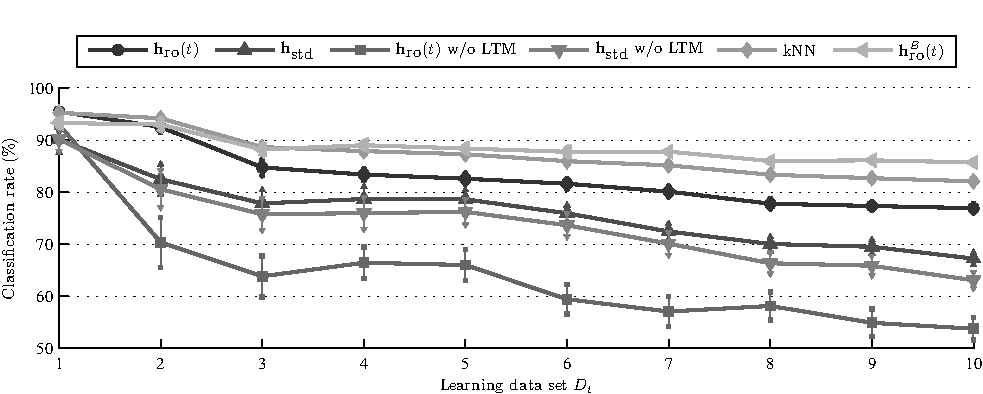
\includegraphics[width=0.98\linewidth]{c1_fig5_1} \label{fig:c1_AddExtErr} }
  \\
  \subfloat[Compression]{
 	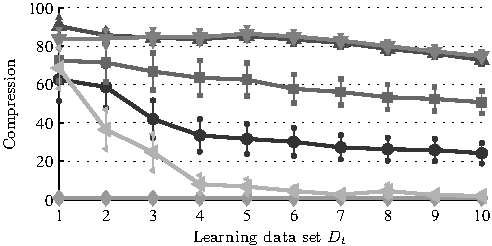
\includegraphics[width=0.46\linewidth]{c1_fig5_2} \label{fig:c1_AddExtCpn} }
   \subfloat[Convergence time]{
 	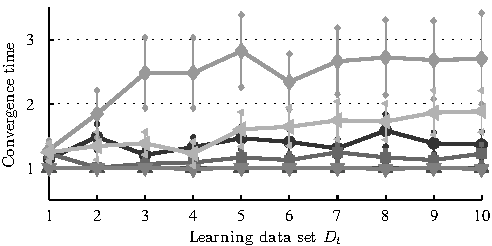
\includegraphics[width=0.46\linewidth]{c1_fig5_3} \label{fig:c1_AddExtEpo} }
	\end{minipage} }
  \caption{Average classification rate, compression, and convergence time of the ACS versus learning block during the enrollment scenario. Performance was evaluated with and without LTM for $\textbf{h}_\text{ro}(t)$ and $\textbf{h}_\text{std}$. Error bars correspond to the 90\% confidence interval. The performance for fuzzy ARTMAP with $\textbf{h}_\text{ro}^B(t)$ and \textit{k}NN during batch learning are shown for reference}
	\label{fig:c1_AddExt}
\end{figure}
%------------------------------------------------------------------------------%

As the amount of training data and the complexity of the decision boundaries increase, all hyperparameters settings follow the same degradation in classification rate. After learning all data, the highest performance is obtained with batch learning (85.6$\pm$0.3\% for $\textbf{h}_\text{ro}^B(t)$ and 82.3$\pm$0.1\% for \textit{k}NN), followed by incremental learning with $\textbf{h}_\text{ro}(t)$ and the LTM (77$\pm$1\%), $\textbf{h}_\text{std}$ with and without the LTM (67$\pm$1\% and 63$\pm$2\%), and finally $\textbf{h}_\text{ro}(t)$ without the LTM (54$\pm$2\%).

However, higher classification rate comes with a cost. Figure \ref{fig:c1_AddExtCpn} shows that compression, when using $\textbf{h}_\text{ro}(t)$ with the LTM starts lower than that obtained without LTM (63$\pm$11 versus 69$\pm$11), decreases to 32$\pm$8 at $D_5$ (compared to 63$\pm$9 without the LTM), and does not change significantly afterwards. Moreover, the average number of training epochs needed when using LTM (1.4$\pm$0.1) is higher than that of $\textbf{h}_\text{ro}(t)$ without LTM (1.1$\pm$0.1), confirming that using a LTM with larger data sets for validation leads to a greater number of training epochs (Figure \ref{fig:c1_AddExtEpo}).

Figure \ref{fig:c1_AddExt} also underline the necessity of storing validation data from all classes when fuzzy ARTMAP is trained with $\textbf{h}_\text{std}$. The networks selected when using LTM are more accurate, yet only more complex on $D_1$, compared to networks selected without the LTM. After incremental learning of 10 blocks with $\textbf{h}_\text{std}$ and LTM, classification rate is 5$\pm$4\% higher and compression is comparable to that obtained with $\textbf{h}_\text{std}$ without LTM. In both cases, convergence time with $\textbf{h}_\text{std}$ is one.
For fuzzy ARTMAP trained with $\textbf{h}_\text{ro}(t)$ and without LTM, Table \ref{tab:c1_AddEvo} shows that since $D_t^\text{f}$, where $2\leq t\leq10$, is only composed of one class ($C_{k'}(t)$), optimization is performed according to that class at the expense of all others ($\{C_k(t)\in \Omega|k\neq k'\}$).
While the classification rate for the class learned at a time $t$, $C_{k'}(t)$, is typically high (above 80\%, except for classes $C_2$ and $C_5$), the average overall classification rate for $\{C_k(t)\in \Omega|k\neq k'\}$ degrades considerably (ends at about $54\%$ after $D_{10}$).
In contrast, by estimating the fitness with LTM, PSO optimization is performed according to all classes and, although classification rate for $C_{k'}(t)$ is lower than without the LTM for all learning blocks, it is always significantly higher for $\{C_k^t\in \Omega|k\neq k'\}$.

%-------------- Classification rate per class for learned class ---------------%
\begin{table}[t]
  \small
  \centering
  \caption{Average classification rate achieved by the ACS for the added classes with each learning block $D_t$ for one class presentation order during the enrollment scenario. The classification rate of the new class added with $D_t$ ($C_{k'}(t)$) is presented with that of the remaining classes present at that time ($\{C_k^t\in \Omega|k\neq k'\}$). Each cell is presented in percentage and with the 90\% confidence interval}
  \begin{tabular}{|l|l|lllllllll|}
  	\hline
		%-- Header
		Training & $D_t$ & $D_{2}$ & $D_{3}$ & $D_{4}$ & $D_{5}$ & $D_{6}$ & $D_{7}$ & $D_{8}$ & $D_{9}$ & $D_{10}$\\\cline{2-11}
		strategy & $C_{k'}(t)$ &  11 &  5 &  4 &  8 &  9 &  7 &  3 &  6 &  2
		\\ \hline \hline

		%-- Hrop w/ LTM
		 & Class. rate for & 90 & 84 & 95 & 99 & 71 & 75 & 68 & 89 & 49	\\ 
		$\textbf{h}_\textnormal{ro}(t)$ & $C_{k'}(t)$ & $\pm 6$ &$\pm 5$ &$\pm 4$ &$\pm 1$ &$\pm 8$ &$\pm 5$ & $\pm 7$ & $\pm 4$ & $\pm 5$	\\ \cline{2-11} 
		w/ LTM &  Class. rate for & 94 & 76 & 79 & 80 & 82 & 79 & 78 & 76 & 77 \\ 
		& $\{C_{k'}(t)\in\Omega|k\neq k'\}$ & $\pm 1$ & $\pm 4$ & $\pm 3$ & $\pm 2$
		& $\pm 2$ & $\pm 2$ & $\pm 2$ & $\pm 2$ & $\pm 2$
		\\ \hline
		
		%-- Hrop w/o LTM
		 & Class. rate for & 100 & 95 & 96 & 98 & 87 & 88 & 77 & 91 & 72 \\ 
		$\textbf{h}_\textnormal{ro}(t)$ & $C_{k'}(t)$ & $\pm 1$ & $\pm 2$ & $\pm 2$ & $\pm 1$ & $\pm 4$ & $\pm 4$ & $\pm 13$ & $\pm 7$ & $\pm 11$	\\ \cline{2-11} 
		w/o LTM & Class. rate for & 31 & 36 & 54 & 61 & 48 & 51 & 56 & 47 & 52 \\ 
		& $\{C_{k'}(t)\in\Omega|k\neq k'\}$ &$\pm 22$ &$\pm 16$ &$\pm 10$ &$\pm 8$
		& $\pm 6$ & $\pm 9$ & $\pm 9$ & $\pm 6$ & $\pm 6$
		\\ \hline
	\end{tabular}
	\label{tab:c1_AddEvo}
\end{table}
%------------- /Classification rate per class for learned class ---------------%

%------------------------ Classification rate per class -----------------------%
\begin{table*}[tb]
  \small
  \centering
  \caption{Average classification rate per class for one class order presentation of the enrollment incremental learning scenario for $\textbf{h}_\text{ro}(t)$ and $\textbf{h}_\text{std}$, with and without the LTM. Results are obtained after enrollment of all classes $C_k\in\Omega$. Each cell is presents the classification rate in percentage along with the 90\% confidence interval}
  \footnotesize{
  \begin{tabular}{|l|lllllllllll|l|}
  	\hline
    Training &\multicolumn{11}{l|}{$C_k \in \Omega$} &\multirow{2}{*}{$\Omega$}
    \\ \cline{2-12}
    strategy &{\bf 1} &{\bf 2} &{\bf 3}  &{\bf 4}  &{\bf 5} & 
    {\bf 6} &{\bf 7} &{\bf 8} &{\bf 9} &{\bf 10} &{\bf 11} &
    \\ \hline \hline
		\multirow{2}{*}{$\textbf{h}_\text{ro}(t)$ w/ LTM}
		& 85 & 49 & 91 & 73 & 49 & 88 & 81 & 70 & 82 & 61 & 91 & 77
		\\ 
 		& $\pm 5$ & $\pm 5$ & $\pm 5$ & $\pm 4$ & $\pm 9$ & $\pm 5$ & $\pm 4$
 		& $\pm 7$ & $\pm 4$ & $\pm 7$ & $\pm 3$ & $\pm 1$
 		\\ \hline 
		\multirow{2}{*}{$\textbf{h}_\text{std}$ w/ LTM}
		& 62 & 5 & 84 & 56 & 93 & 78 & 67 & 32 & 83 & 37 & 77 & 67
		\\ 
		& $\pm 24$ & $\pm 4$ & $\pm 5$ & $\pm 6$ & $\pm 6$ & $\pm 4$ & $\pm 5$
		& $\pm 7$ & $\pm 2$ & $\pm 7$ & $\pm 4$ & $\pm 1$
		\\ \hline \hline 
		\multirow{2}{*}{$\textbf{h}_\text{ro}(t)$ w/o LTM}
		& 62 & 72 & 45 & 66 & 21 & 73 & 61 & 37 & 67 & 47 & 39 & 54
		\\ 
		& $\pm 24$ & $\pm 11$ & $\pm 25$ & $\pm 19$ & $\pm 19$ & $\pm 21$ 
		& $\pm 17$ & $\pm 25$ & $\pm 12$ & $\pm 17$ & $\pm 25$ & $\pm 2$
		\\ \hline 
		\multirow{2}{*}{$\textbf{h}_\text{std}$ w/o LTM}
		& 36 & 7 & 81 & 47 & 87 & 78 & 68 & 43 & 81 & 40 & 75 & 63
		\\ 
		& $\pm 8$ & $\pm 5$ & $\pm 8$ & $\pm 10$ & $\pm 7$ & $\pm 5$ & $\pm 7$
		& $\pm 11$ & $\pm 4$ & $\pm 7$ & $\pm 6$ & $\pm 2$
		\\ \hline 
	\end{tabular} }
	\label{tab:c1_AddExt}
\end{table*}
%------------------------ Classification rate per class -----------------------%

As mentioned, when the decision boundaries between class distributions are complex, it is difficult for the ACS to maintain a high classification rate with compact fuzzy ARTMAP networks. As classes are added to the ACS using $\textbf{h}_\text{std}$, the recognition categories created for new classes tend to expand into the boundaries of the older class distributions. The order in which classes are learned may then prove crucial for optimal performance. With the class presentation order given in Table \ref{tab:c1_AddEvo} and Table \ref{tab:c1_AddExt}, excepted for class $C_2$, which contains only 39 learning patterns, classification rates obtained for the latest classes added to the system using $\textbf{h}_\text{ro}(t)$ with LTM (classes $C_3$, $C_6$, $C_7$, and $C_9$) is significantly higher than those obtained using without LTM. The performance of these later classes are obtained at the expense of those present in previous blocks. However, no matter the choice of hyperparameters, classes $C_1$ and $C_3$ are not greatly affected by the addition of latter classes, suggesting that data distributions of classes $C_1$ and $C_3$ do not overlap those of classes $C_3$, $C_6$, $C_7$, and $C_9$.

%------------------------------------------------------------------------------%
%------------------------------------------------------------------------------%
\subsubsection{Update scenario}

%------------------------------------------------------------------------------%
\begin{figure*}[!t]
  \centering
	\fbox{\begin{minipage}{0.97\linewidth}\centering
  \subfloat[Classification rate]{
  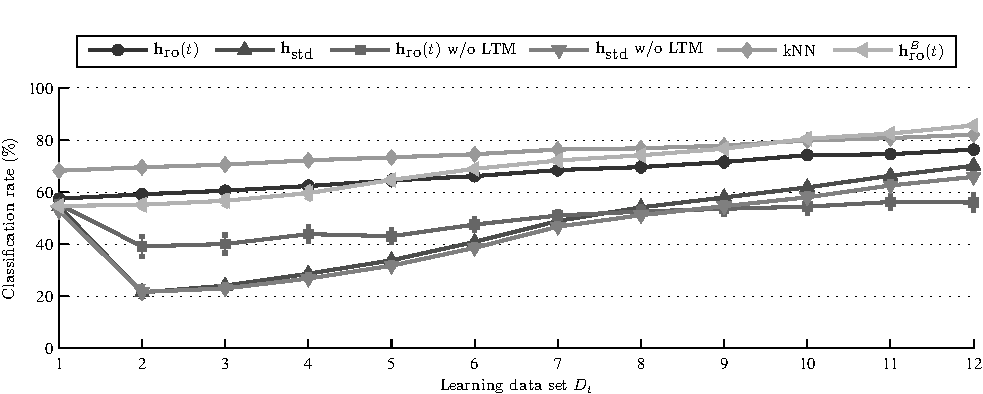
\includegraphics[width=0.98\linewidth]{c1_fig6_1} \label{fig:c1_RefExtErr} }
	\\
	\subfloat[Compression]{
  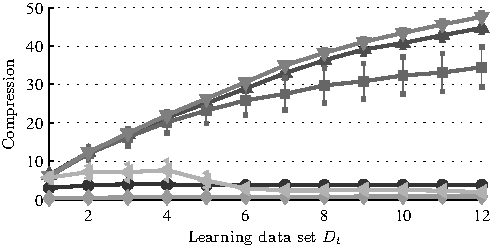
\includegraphics[width=0.48\linewidth]{c1_fig6_2} \label{fig:c1_RefExtCpn} }
  \subfloat[Convergence time]{
  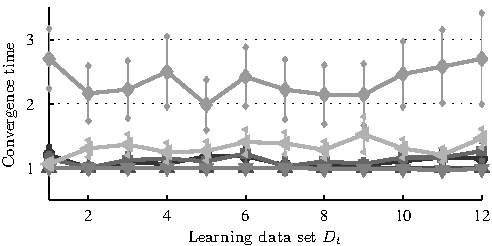
\includegraphics[width=0.48\linewidth]{c1_fig6_3} \label{fig:c1_RefExtEpo} }
	\end{minipage} }
 	\caption{Average classification rate, compression, and convergence time of the ACS versus learning block during the update scenario. Performance was evaluated with and without LTM for $\textbf{h}_\text{ro}(t)$ and $\textbf{h}_\text{std}$. Error bars correspond to the 90\% confidence interval. The performance for fuzzy ARTMAP with $\textbf{h}_\text{ro}^B(t)$ and \textit{k}NN during batch learning are shown for reference}
	\label{fig:c1_RefExt}
\end{figure*}
%------------------------------------------------------------------------------%

In the update scenario, all classes are defined from the start in $D_1$ with only 10\% of the available learning data. While \textit{k}NN yields a classification rate of 68.1$\pm$0.4 after learning $D_1$, the classification rate of the ACS for all system parameters settings starts below 60\%. This indicates that decision boundaries are very complex, and learning $D_1$ with limited data from each class is a difficult task for the ACS. As it was presented in \cite{granger08, connolly08}, this shows the importance of $D_1$ when fuzzy ARTMAP undergoes incremental learning, as it forms the basis for future updates with video data. An ACS should then be initiated with enough representative data from the environment.

At the beginning of the update process ($t \leq 4$), using more validation data with the LTM results in an increase in classification rates of the ACS when $\textbf{h}_\text{ro}(t)$ is used during incremental learning. Moreover, the ACS with $\textbf{h}_\text{ro}(t)$ and LTM gives a similar classification rate as the reference systems, minus the effects of knowledge corruption. While the classification rate with $\textbf{h}_\text{ro}(t)$ starts at 57.4$\pm$0.5\% at $t=1$ and steadily increases up to 76$\pm$1\% at $t=10$, classification rate with View the MathML source starts at 55$\pm$1\%, reaches 60$\pm$2\% at $t=4$, and increases faster than that of $\textbf{h}_\text{ro}(t)$ to end at 85.6$\pm$0.3\%. This sudden increase in performance also correspond to a decrease in compression. While compression of $\textbf{h}_\text{ro}(t)$ starts at 3$\pm$1 at $t=1$ and remains steady at 4$\pm$1 for $ 2\leq t \leq12$, compression of $\textbf{h}_\text{ro}^B(t)$ increases from 6$\pm$1 ($t=1$) to 8$\pm$2 ($t=4$), and suddenly drops to 2.4$\pm$0.4 ($t=7$) without changing significantly afterwards. Overall, $\textbf{h}_\text{ro}^B(t)$ needed about 1.7 more nodes than $\textbf{h}_\text{ro}(t)$ to obtained a classification rate 10\% higher. It outperforms \textit{k}NN classification rate, compression, and convergence time.

Meanwhile, classification rates obtained with $\textbf{h}_\text{std}$ and $\textbf{h}_\text{ro}(t)$ (without LTM) decrease considerably $t=2$ (22$\pm$2\% for both cases of $\textbf{h}_\text{std}$ and to 39$\pm$4\% for $\textbf{h}_\text{ro}(t)$ without LTM). However, updating all classes using $\textbf{h}_\text{std}$ increases overall performances (classification rate increases by about 15\% with LTM, 13\% without LTM, and with a higher compression in both cases), while using $\textbf{h}_\text{ro}(t)$ without LTM only results in a gain in compression (classification rates after learning $D_1$ and $D_{12}$ that are both 59$\pm$2\%).

As with the enrollment learning scenario, Table \ref{tab:c1_RefEvo} shows that the ACS without the LTM is only optimized for classes updated with each $D_t$. Classification rates for $C_{k'}(t)$ are either higher than or comparable to those of $\textbf{h}_\text{ro}(t)$ with the LTM, while the classification rates for $\{C_k(t)\in \Omega|k\neq k'\}$ are degraded compared to those obtained when using the LTM. Coarse decision boundaries created at the beginning of the update process ($D_2$) are refined when new data becomes available. As the overall classification rate increases, the difference between $C_{k'}(t)$ and $\{C_k(t)\in \Omega|k\neq k'\}$ decreases (from 45$\pm$5\% at $t=2$, to 19$\pm$7\% at $t=12$).

Unlike with the enrollment scenario, Table \ref{tab:c1_RefEvo} and Table \ref{tab:c1_RefExt} show that individual classification rates obtained after learning all data are less sensitive to class order presentation when all classes defined in $D_1$. Classification rates of $C_{k'}(t)$ obtained with $\textbf{h}_\text{ro}(t)$ and LTM in Table \ref{tab:c1_RefEvo} are no longer systematically below those of $\textbf{h}_\text{ro}(t)$ without LTM. Moreover, individual classification rates from Table \ref{tab:c1_RefExt} differ less from the overall classification rate and their dispersion is lower. As an example, $\textbf{h}_\text{ro}(t)$ with LTM yield a standard deviation of 16 for the individual classification rates during the enrollment scenario, and a standard deviation of 14 for the update scenario. This lead to higher global classification rates over all classes.

%-------------- Classification rate per class for learned class ---------------%
\begin{center}
\begin{table*}[tb]
  \small
  \centering
  \caption{Average classification rate achieved by the ACS for the updated classes with each learning block $D_t$ for one class presentation order during the update scenario. The classification rate of the updated class with $D_t$ ($C_{k'}(t)$) is presented with that of the remaining classes ($\{C_k^t\in \Omega|k\neq k'\}$). Each cell is presented in percentage and with the 90\% confidence interval}
  \footnotesize{
  \begin{tabular}{|l|l|lllllllllll|}
  \hline
	%-- Header
	Training & $D_t$ & $D_{2}$ & $D_{3}$ & $D_{4}$ & $D_{5}$ & $D_{6}$ & $D_{7}$ & $D_{8}$ & $D_{9}$ & $D_{10}$ & $D_{11}$ & $D_{12}$	\\ \cline{2-13}
	strategy & $C_{k'}(t)$ & 11 & 5 & 1 & 7 & 9 & 3 & 10 & 4 & 8 & 6 & 2
	\\ \hline \hline

	%-- Hrop w/ LTM
	 & Class. rate for & 90 & 77 & 98 & 88 & 87 & 98 & 78 & 87 & 70 & 92 & 92
	\\ 
	$\textbf{h}_\textnormal{ro}(t)$ & $C_{k'}(t)$ & $\pm$4 & $\pm$6 & $\pm$2 & $\pm$3 & $\pm$5 & $\pm$1	& $\pm$7 & $\pm$6 & $\pm$12 & $\pm$4 & $\pm$4
	\\ \cline{2-13} 
	w/ LTM & Class. rate for & 55 & 62 & 60 & 64 & 68 & 65 & 70 & 74 & 76 & 74 & 73
	\\ 
	 & $\{C_{k'}(t)\in\Omega|k\neq k'\}$ & $\pm$1 & $\pm$1 & $\pm$1 & $\pm$2
	& $\pm$2 & $\pm$3 & $\pm$2 & $\pm$3 & $\pm$3 & $\pm$3 & $\pm$3
	\\ \hline \hline
	%-- Hrop w/0 LTM
	 & Class. rate for & 98 & 86 & 95 & 82 & 91 & 99 & 80 & 85 & 72 & 90 & 74 \\ 
	 $\textbf{h}_\textnormal{ro}(t)$ & $C_{k'}(t)$ & $\pm$2 & $\pm$7 & $\pm$3 & $\pm$8 & $\pm$2 & $\pm$1 & $\pm$7 & $\pm$7 & $\pm$13 & $\pm$5 & $\pm$13	\\ \cline{2-13} 
	w/o LTM & Class. rate for & 37 & 32 & 36 & 39 & 43 & 46 & 50 & 51 & 51 & 59 & 51 \\ 
	& $\{C_{k'}(t)\in\Omega|k\neq k'\}$ & $\pm$8 & $\pm$10 & $\pm$6 & $\pm$6
	& $\pm$6 & $\pm$4 & $\pm$5 & $\pm$7 & $\pm$8 & $\pm$7 & $\pm$10
	\\ \hline

	\end{tabular} }
	\label{tab:c1_RefEvo}
\end{table*}
\end{center}
%-------------- Classification rate per class for learned class ---------------%

%------------------------ Classification rate per class -----------------------%
\begin{table*}[tb]
  \small
  \centering
  \caption{Average classification rate per class for one class order presentation of the update incremental learning scenario for $\textbf{h}_\text{ro}(t)$ and $\textbf{h}_\text{std}$, with and without the LTM. Results are obtained after update of all classes $C_k\in\Omega$. Each cell is presents the classification rate in percentage along with the 90\% confidence interval}
  \footnotesize{
  \begin{tabular}{|l|lllllllllll|l|} \hline
    Training &\multicolumn{11}{l|}{$C_k \in \Omega$} &\multirow{2}{*}{$\Omega$}
    \\ \cline{2-12}
    strategy &{\bf 1} &{\bf 2} &{\bf 3}  &{\bf 4}  &{\bf 5} & 
    {\bf 6} &{\bf 7} &{\bf 8} &{\bf 9} &{\bf 10} &{\bf 11} &
    \\ \hline \hline
		\multirow{2}{*}{$\textbf{h}_\text{ro}(t)$ w/ LTM}
		& 83 & 92 & 92 & 82 & 53 & 92 & 82 & 69 & 70 & 59 & 60 & 76
		\\ 
		& $\pm 8$ & $\pm 5$ & $\pm 5$ & $\pm 8$ & $\pm 8$ & $\pm 4$ & $\pm 2$
		& $\pm 12$ & $\pm 14$ & $\pm 7$ & $\pm 11$ & $\pm 1$
		\\ \hline 
		\multirow{2}{*}{$\textbf{h}_\text{std}$ w/ LTM} 
		& 57 & 11 & 94 & 38 & 83 & 85 & 78 & 34 & 84 & 52 & 78 & 70
		\\ 
		& $\pm 28$ & $\pm 5$ & $\pm 3$ & $\pm 9$ & $\pm 5$ & $\pm 5$ & $\pm 6$
		& $\pm 6$ & $\pm 2$ & $\pm 5$ & $\pm 4$ & $\pm 1$
		\\ \hline \hline
		\multirow{2}{*}{$\textbf{h}_\text{ro}(t)$ w/o LTM}
		& 57 & 74 & 54 & 59 & 18 & 56 & 52 & 69 & 72 & 41 & 44 & 56
		\\ 
		& $\pm 28$ & $\pm 14$ & $\pm 27$ & $\pm 25$ & $\pm 15$ & $\pm 25$ 
		& $\pm 20$ & $\pm 18$ & $\pm 12$ & $\pm 19$ & $\pm 25$ & $\pm 3$
		\\ \hline 
		\multirow{2}{*}{$\textbf{h}_\text{std}$ w/o LTM} 
		& 38 & 3 & 84 & 38 & 89 & 83 & 70 & 44 & 81 & 38 & 71 & 66
		\\ 
		& $\pm 8$ & $\pm 3$ & $\pm 6$ & $\pm 9$ & $\pm 8$ & $\pm 5$ & $\pm 7$
		& $\pm 7$ & $\pm 3$ & $\pm 7$ & $\pm 6$ & $\pm 2$
		\\ \hline 
	
	\end{tabular} }
	\label{tab:c1_RefExt}
\end{table*}
%------------------------ Classification rate per class -----------------------%

%------------------------------------------------------------------------------%
%------------------------------------------------------------------------------%
\subsection{Experiment ($B$) -- Impact of dynamic optimization}

Figure \ref{fig:c1_AddDyn} and Figure \ref{fig:c1_RefDyn} present the average classification rate, compression, and convergence time achieved by the ACS with a LTM and with system parameters that are optimized using: dynamic optimization with DNPSO ($\textbf{h}_\text{dnc}(t)$), DNPSO on only $D_1$ and are then fixed ($\textbf{h}_\text{dnc}(1)$), static optimization with DNPSO ($\textbf{h}_\text{stc}(t)$), static optimization with canonical PSO ($\textbf{h}_\text{cnl}(t)$), and the reference batch learning method ($\textbf{h}_\text{ro}^B(t)$). The evolution of hyperparameters found via $\textbf{h}_\text{dnc}(t)$ is shown for all class presentation order in Figure \ref{fig:c1_AddDynHp} and Figure \ref{fig:c1_RefDynHp} after incremental learning of different blocks for both incremental learning scenario. Figure \ref{fig:c1_AddDynSwarm} and Figure \ref{fig:c1_RefDynSwarm} shows the position of the swarms at different moments in time for the same class presentation order used in Table \ref{tab:c1_AddEvo}, Table \ref{tab:c1_AddExt}, Table \ref{tab:c1_RefEvo} and Table \ref{tab:c1_RefExt}.

%------------------------------------------------------------------------------%
\subsubsection{Enrollment scenario}

%--------------------------- Perfomances - Addition ---------------------------%
\begin{figure}[!b]
  \centering
	\fbox{\begin{minipage}{0.97\linewidth}\centering
  \subfloat[Classification rate]{
 	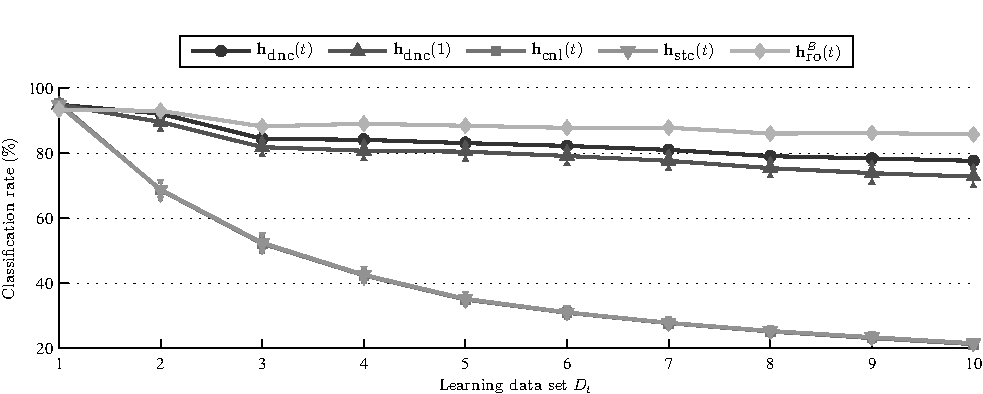
\includegraphics[width=0.98\linewidth]{c1_fig7_1} \label{fig:c1_AddDynErr} }
  \\
  \subfloat[Compression]{
 	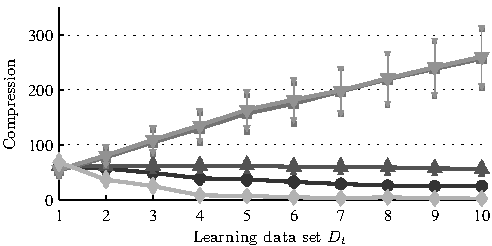
\includegraphics[width=0.48\linewidth]{c1_fig7_2} \label{fig:c1_AddDynCpn} }
  \subfloat[Convergence time]{
 	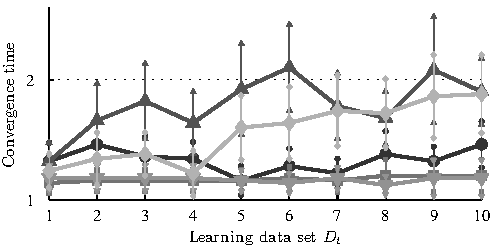
\includegraphics[width=0.48\linewidth]{c1_fig7_3} \label{fig:c1_AddDynEpo} }
	\end{minipage} }
  \caption{Average classification rate, compression, and convergence time of the ACS versus learning block during the enrollment scenario. Performance was evaluated with the LTM for $\textbf{h}_\text{dnc}(t)$, $\textbf{h}_\text{dnc}(1)$, $\textbf{h}_\text{stc}(t)$, and $\textbf{h}_\text{cnl}(t)$. Error bars correspond to the 90\% confidence interval. The performance for fuzzy ARTMAP with $\textbf{h}_\text{ro}^B(t)$ during batch learning is shown for reference}
	\label{fig:c1_AddDyn}
\end{figure}
%--------------------------- Perfomances - Addition ---------------------------%

Figure \ref{fig:c1_AddDyn} illustrates that, when the proposed ACS is used with a static optimization algorithm ($\textbf{h}_\text{stc}(t)$ and $\textbf{h}_\text{cnl}(t)$), classification rate declines significantly during the enrollment learning scenario. Unlike with dynamic optimization ($\textbf{h}_\text{dnc}(t)$), static optimization algorithms does not automatically update the fitness corresponding to the position of each particle's personal best when a new $D_t$ becomes available, requiring the $\textit{FAM}_n$ networks to be trained on $D_t^\text{t}$ (Line \ref{l:c1_trnUpdate}). As classes are added to the ACS, decision boundaries become more complex and fitness values estimated on $D_t^\text{f}$, initially 100\% after learning $D_1$, decline in time. The particle's personal best positions of static PSO algorithms ($\textbf{h}_\text{stc}(t)$ and $\textbf{h}_\text{cnl}(t)$) are thus never redefined, and the $\textit{FAM}_n$ networks, which learn two classes on $D_1$, are never updated afterwards. The rest of the learning process is then always based on a $\textit{FAM}_n$ neural network that learned only two classes.

When using a dynamic PSO algorithm, Figure \ref{fig:c1_AddDynHp} shows that $\textbf{h}_\text{dnc}(t)$ changes such that fuzzy ARTMAP can maintain a higher classification rate with low confidence interval. Although the confidence interval for all hyperparameters tends to be large, Figure \ref{fig:c1_AddDynHp} still indicates that they vary according to some pattern no matter class presentation order. Moreover, the impact of new data on fuzzy ARTMAP hyperparameters does not appear to diminished as more classes are presented to ACS with $\textbf{h}_\text{dnc}(t)$.

%-------------------------- HP evolution - Addition ---------------------------%
\begin{figure}[t]
  \centering
	\fbox{
 	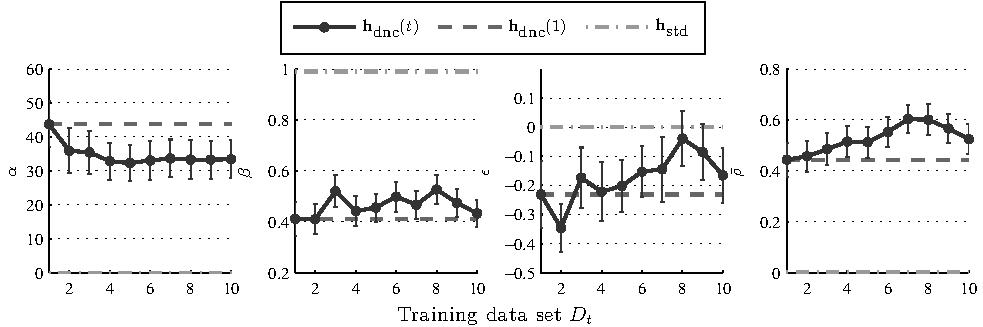
\includegraphics[width=0.97\linewidth]{c1_fig8}
 	}
  \caption{ Evolution of hyperparameter values obtained with the ACS using $\textbf{h}_\text{dnc}(t)$ compared to the ACS based on $\textbf{h}_\text{dnc}(t)$ and $\textbf{h}_\text{std}$(t) during the enrollment scenario. The mean of each hyperparameter is shown with its 90\% confidence interval}
	\label{fig:c1_AddDynHp}
\end{figure}
%-------------------------- HP evolution - Addition ---------------------------%

While $\alpha$ changes significantly only once from 44$\pm$7 at $t=1$ to 36$\pm$7 at $t=2$, $\beta$ starts at 0.40$\pm$0.07 and changes significantly four times at $t\in\{3,4,8,9\}$ (to 0.52$\pm$0.06, 0.44$\pm$0.06, 0.53$\pm$0.06, and 0.43$\pm$0.06). Hyperparameter $\epsilon$ starts at $-0.23\pm$0.11 and changes four times at $t\in\{2,3,8,10\}$ (to $-0.35\pm$0.08, $-0.17\pm$0.10, $-0.04\pm$0.09, and $-0.17\pm$0.09). Finally, $\bar{\rho}$  starts at 0.44$\pm$0.07, increases to 0.60$\pm$0.05 at $t=7$ and decreases to 0.52$\pm$0.06. Figure \ref{fig:c1_AddDynSwarm} shows the evolution of particles in the DNPSO swarm mapped in two dimensions space using Sammon's mapping (\cite{kim09}). As expected, the classification rates estimated for most of the networks after $D_1$ are 100\%. As classes are added to the system, DNPSO subswarms moves in the hyperparameters space as new peaks appear and disappear in the objective function. Even if the global best solution obtained during incremental learning is not always near the global best obtained with $\textbf{h}_\text{ro}^B(t)$, the latter is always found by one of the DNPSO subswarms. This indicates that the optimization space defined by fuzzy ARTMAP hyperparameters adjustment for the enrollment scenario does in fact correspond to a type III optimization environment (see Section \ref{sec:c1_adaptation}).

%--------------------------- HP evolution - Addition --------------------------%
\begin{figure}[t]
  \centering
	\fbox{ 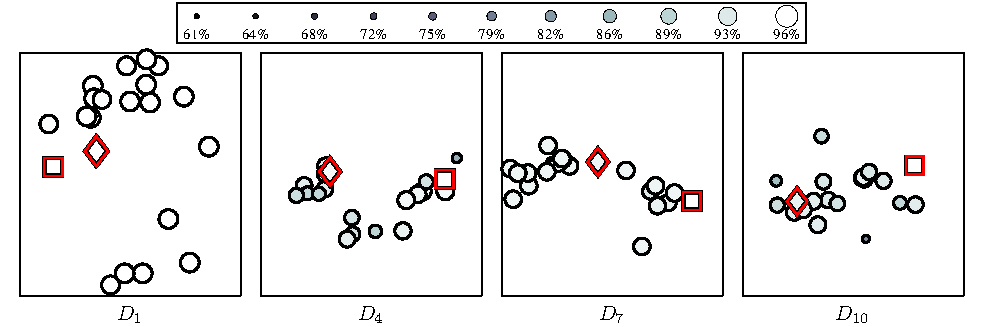
\includegraphics[width=0.97\linewidth]{c1_fig9} }
	\caption{A two-dimensional Sammon's mapping illustrating the evolution of each particle's personal best, and the swarm's global best positions when the proposed ACS performs incremental learning with $\textbf{h}_\text{dnc}(t)$ (diamond) for the enrollment scenario. The global best particle position obtained for batch learning with $\textbf{h}_\text{ro}^B(t)$ (square) is also shown for reference. Positions are shown along the estimation of $f(\textbf{h},t)$ (see legend) when the optimization stopping conditions have been reached for different points in time ($t\in\{1,4,7,10\}$) during the update scenario for one replication and the same class presentation order presented in the previous sections}
	\label{fig:c1_AddDynSwarm}
\end{figure}
%-------------------------- HP evolution - Addition ---------------------------%

Beside the reference $\textbf{h}_\text{ro}^B(t)$, the ACS based on $\textbf{h}_\text{dnc}(t)$ achieves the highest (78$\pm$1\%), followed by $\textbf{h}_\text{dnc}(1)$ (72$\pm$3\%), $\textbf{h}_\text{stc}(t)$, and $\textbf{h}_\text{cnl}(t)$ (both at 21$\pm$1\%). Compared to $\textbf{h}_\text{dnc}(1)$, classification rates with $\textbf{h}_\text{dnc}(t)$ starts 94.8$\pm$0.6\% and become significantly different to that of $\textbf{h}_\text{dnc}(1)$ as of $t=2$. As in previous results, a lower compression (25$\pm$1 at $t=10$) is necessary to maintain higher classification rates.

Results with the MoBo data base confirms the results obtained with the IIT-NRC data base. However, since the acquisition of the MoBo data is more constrained than that of the IIT-NRC data, class distributions $p_k(\textbf{a})$ are more compact and are less likely to vary significantly from one block to the next. As Table \ref{tab:c1_AddMobo} shows, classification rates are comparable for $\textbf{h}_\text{dnc}(t)$ and $\textbf{h}_\text{dnc}(1)$, and compressions are twice as high as those obtained with the IIT-NRC data base.

%------------------------------- Results - MoBo -------------------------------%
\begin{table*}[tb]
  \small
  \centering
  \caption{Average classification rate (in percentage) and compression after incremental learning of all the MoBo data base for the enrollment scenario. Each cell is presented with the 90\% confidence interval}
  \begin{tabular*}{\linewidth}{@{\extracolsep{\fill}}|l|llll|}
  	\hline
    Performance indicator      & $\textbf{h}_\text{dnc}(t)$
															 & $\textbf{h}_\text{dnc}(1)$
															 & $\textbf{h}_\text{stc}(t)$
															 & $\textbf{h}_\text{cnl}(t)$
    \\ \hline 
    Classification rate & $79\pm2\%$ & $78\pm4\%$ & $20\pm1\%$ & $20\pm1\%$
    \\ 
    Compression         & $45\pm3$ & $97\pm80$ & $480\pm10$ & $480\pm10$
    \\ \hline
	\end{tabular*}
	\label{tab:c1_AddMobo}
\end{table*}
%------------------------------- Results - MoBo -------------------------------%

%------------------------------------------------------------------------------%
%------------------------------------------------------------------------------%
\subsubsection{Update scenario}

%------------------------------------------------------------------------------%
\begin{figure}[!t]
  \centering
	\fbox{\begin{minipage}{0.97\linewidth}\centering
   \subfloat[Classification rate]{
 		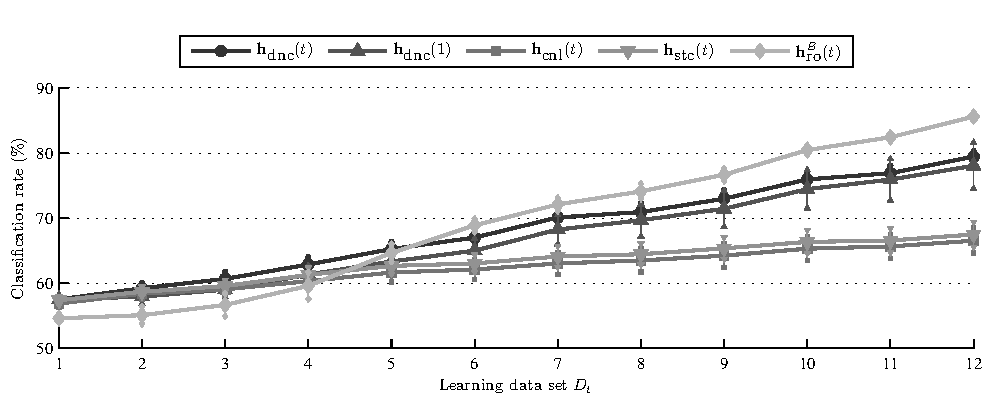
\includegraphics[width=0.98\linewidth]{c1_fig10_1} \label{fig:c1_RefDynErr} }
  \\
  \subfloat[Compression]{
 		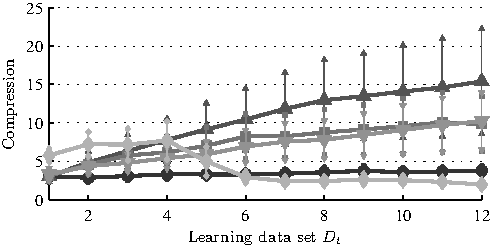
\includegraphics[width=0.48\linewidth]{c1_fig10_2} \label{fig:c1_RefDynCpn} }
  \subfloat[Convergence time]{
 		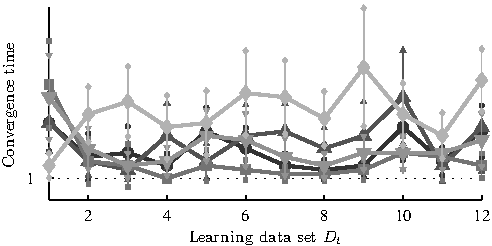
\includegraphics[width=0.48\linewidth]{c1_fig10_3} \label{fig:c1_RefDynEpo} }
	\end{minipage} }
	\caption{Average classification rate, compression, and convergence time of the ACS versus learning block during the update scenario. Performance was evaluated with the LTM for $\textbf{h}_\text{dnc}(t)$, $\textbf{h}_\text{dnc}(1)$, $\textbf{h}_\text{stc}(t)$, and $\textbf{h}_\text{cnl}(t)$. Error bars correspond to the 90\% confidence interval. The performance for fuzzy ARTMAP with $\textbf{h}_\text{ro}^B(t)$ during batch learning is shown for reference}
	\label{fig:c1_RefDyn}
\end{figure}
%------------------------------------------------------------------------------%


Figure \ref{fig:c1_RefDyn} also shows that using an ACS based on static optimization algorithms ($\textbf{h}_\text{stc}(t)$ and $\textbf{h}_\text{cnl}(t)$) results in poor incremental learning capabilities. In some cases, both DNPSO, applied without updating the personal best when new data is available ($\textbf{h}_\text{stc}(t)$), and canonical PSO ($\textbf{h}_\text{cnl}(t)$) algorithms find an hyperparameter vector that remains an optimum through during the entire learning process. But in other cases, the swarm stays in a region of the optimization space where classification rate does not improve and, as with the enrollment scenario, fitness corresponding to personal best positions does not improve and the $\textit{FAM}_n$ neural networks are never updated. Since the DNPSO algorithm, used without updating the personal best, is able to maintain diversity in the optimization space, it tends to provide a higher level of performance after learning all data but shows no significant differences with canonical PSO (68$\pm$2\% for $\textbf{h}_\text{stc}(t)$ versus 67$\pm$2\% $\textbf{h}_\text{cnl}(t)$). In both cases the average classification rate remains below 70\%.

As blocks of data are presented to the ACS during the update scenario, Figure \ref{fig:c1_RefDynHp} shows that all four hyperparameters are also adjusted during the update scenario. While, $\alpha$ steadily increases from 49$\pm$7 to 74$\pm$5, $\beta$ significantly changes five times ($t=\{2,5,9,10\}$) with values ranging from 0.26$\pm$0.06 to 0.48$\pm$0.07, $\epsilon$ changes two times ($t=\{2,7\}$) with values ranging from $-0.04\pm0.12$ to 0.11$\pm$0.12 and very high confidence intervals, and $\bar{\rho}$ changes five times ($t=\{2,5,9,10,11\}$) with values ranging from 0.62$\pm$0.08 to 0.82$\pm$0.06.

%--------------------------- HP evolution - Update ----------------------------%
\begin{figure}[ht]
  \centering
	\fbox{ 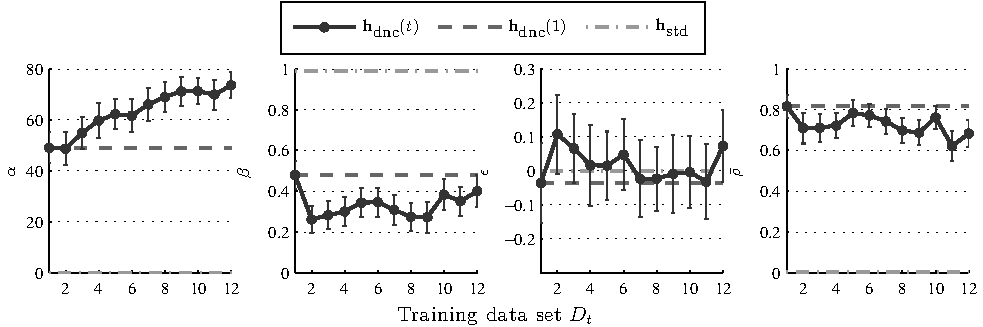
\includegraphics[width=0.97\linewidth]{c1_fig11} }
	\caption{Evolution of hyperparameter values obtained with the ACS using $\textbf{h}_\text{dnc}(t)$ compared to the ACS based on $\textbf{h}_\text{dnc}(t)$ and $\textbf{h}_\text{std}$(t) during the update scenario. The mean of each hyperparameter is shown with its 90\% confidence interval}
	\label{fig:c1_RefDynHp}
\end{figure}
%--------------------------- HP evolution - Update ----------------------------%

Like with the enrollment scenario, when observing the evolution of particles in the DNPSO swarm mapped in two dimensions space using Sammon's mapping, Figure \ref{fig:c1_RefDynSwarm} indicates the presence of a type III dynamic optimization environment (Section \ref{sec:c1_adaptation}). The personal best position of each particle are adjusted in response to peaks in the objective function $f(\textbf{h},t)$ that change position and values in time. However, since all classes are present in $D_1$, most of the feature space is define at the outset of the incremental learning process. Apart from the peak appearing in the middle of the optimization space at $t=4$, most of the changes in $f(\textbf{h},t)$ happen in the interval $4\leq t\leq8$.

%--------------------------- HP evolution - Update ----------------------------%
\begin{figure}[ht]
  \centering
 	\fbox{ 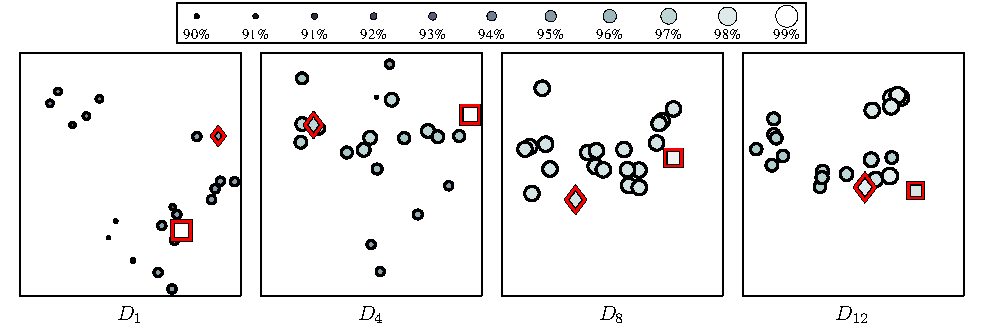
\includegraphics[width=0.97\linewidth]{c1_fig12}	}
	\caption{A two-dimensional Sammon's mapping illustrating the evolution of each particle's personal best, and the swarm's global best positions when the proposed ACS performs incremental learning with $\textbf{h}_\text{dnc}(t)$ (diamond) for the update scenario. The global best particle position obtained for batch learning with $\textbf{h}_\text{ro}^B(t)$ (square) is also shown for reference. Positions are shown along the estimation of $f(\textbf{h},t)$ (see legend) when the optimization stopping conditions have been reached for different points in time ($t\in\{1,4,8,12\}$) during the update scenario for one replication and the same class presentation order presented in the previous sections}
	\label{fig:c1_RefDynSwarm}
\end{figure}
%--------------------------- HP evolution - Update ----------------------------%

For the update scenario, the highest and more stable classification rate is achieved by dynamic optimization with $\textbf{h}_\text{dnc}(t)$ (Figure \ref{fig:c1_RefDyn}). Classification rates starts at 57.5$\pm$0.4\% and end at 79.4$\pm$0.9\%. It is almost always above classification rate obtained with $\textbf{h}_\text{dnc}(1)$ by at least 1\%. As shown in Figure \ref{fig:c1_RefDynCpn}, solutions obtained with $D_1$ are mostly heavy solutions that accommodate a complex input features space containing all classes. For $t>1$, those solutions yield large fuzzy ARTMAP neural networks, similar to those obtain in batch learning, and provide high classification rates. Moreover, the global best positions found at $t=1$ tend to remain in the vicinity of, at least, one subsequent local best position found during incremental learning, and of the global best positions found during batch learning (Figure \ref{fig:c1_RefDynSwarm}).

On the other hand, the ACS with $\textbf{h}_\text{dnc}(1)$ also find lighter solutions that performs also well on $D_1$, but then gives lower classification rate than the ACS with $\textbf{h}_\text{dnc}(t)$ when classes are updated. For $t\geq6$, when batch learning surpass incremental learning, those solutions do not perform as well as the larger ones, and the confidence interval for the classification rate grows from 1.4 at $t=4$ to 3.5 at $t=12$ while the latter for compression eventually grows to 7.

%------------------------------- Results - MoBo -------------------------------%
\begin{table*}[tb]
  \small
  \centering
  \caption{Average classification rate (in percentage) and compression after incremental learning of all the MoBo data base for the update scenario. Each cell is presented with the 90\% confidence interval}
  \begin{tabular*}{\linewidth}{@{\extracolsep{\fill}}|l|llll|}
  	\hline
    Performance indicator      & $\textbf{h}_\text{dnc}(t)$
															 & $\textbf{h}_\text{dnc}(1)$
															 & $\textbf{h}_\text{stc}(t)$
															 & $\textbf{h}_\text{cnl}(t)$
    \\ \hline
    Classification rate & $85\pm2\%$ & $88\pm3\%$ & $51\pm1\%$ & $52\pm1\%$
    \\
    Compression         & $11\pm2$ & $20\pm8$ & $36\pm9$ & $33\pm9$
    \\ \hline
	\end{tabular*}
	\label{tab:c1_RefMobo}
\end{table*}
%------------------------------- Results - MoBo -------------------------------%

Once again, results with the MoBo data base confirms the results obtained with the IIT-NRC data (Table \ref{tab:c1_RefMobo}). Classes in the MoBo data base are found to be more easily updated for $\textbf{h}_\text{dnc}(t)$ and $\textbf{h}_\text{dnc}(1)$. Both classification rates obtained with MoBo are over 5\% higher than those obtain on the IIT-NRC data. Since acquisition conditions are more constrained, $D_1$ data structure is now more representative of the entire learning data set and solutions found with $\textbf{h}_\text{dnc}(1)$ remain comparable to $\textbf{h}_\text{dnc}(t)$ in terms of classification rate. The average compression is also higher for all hyperparameters settings, but as with IIT-NRC, it is higher with $\textbf{h}_\text{dnc}(1)$. ACS using static optimization with MoBo also results in lighter solutions, those solutions yield lower classification rates.

%------------------------------------------------------------------------------%
%--------------------------------- Conclusion ---------------------------------%
\section{Conclusion}

In this chapter, an adaptive classification system (ACS) is proposed for video-based face recognition. It combines a fuzzy ARTMAP neural network classifier, dynamic particle swarm optimization (DPSO) algorithm, and a long term memory (LTM). This ACS uses a novel DPSO-based learning strategy to cojointly optimize the classifier weights, architecture, and user-defined hyperparameters such as classification rate is maximized during incremental learning of new data. This DPSO-based learning strategy reconsiders the four properties of a classification system capable of supervised incremental learning (as defined in \cite{polikar01}) in two ways. The $2^{nd}$ property is modified to include the storage and management of previously acquired learning data for unbiased validation and fitness estimation. To avoid knowledge corruption, and thereby maintain a high level of performance, a $5^{th}$ property is added to the others: a classifier must adapt its learning dynamics by adjusting its hyperparameters.

Using real-world video data bases, performance of this system is assessed in terms of classification rate and resource requirements, for different hyperparameter settings, with and without LTM. Overall results of experiments ($A$) and ($B$) demonstrate that optimizing fuzzy ARTMAP hyperparameters during incremental learning gives higher classification rates than when using standard or fixed hyperparameters ($\textbf{h}_\text{std}$ and $\textbf{h}_\text{dnc}(1)$). When property (5) of an incremental learning algorithm is applied, results indicate that, during incremental learning, fuzzy ARTMAP performance degrades unless some validation data are stored and updated in a LTM. Moreover, experiment ($B$) shows that, as more samples are learned by fuzzy ARTMAP with the LTM, peaks of the objective function (in the hyperparameters space) changes in time. Adjusting hyperparameters during incremental learning thus corresponds to a type III dynamic optimization problem and if a dynamic optimization algorithm is not employed to adjust classifier hyperparameters, then classification rate of fuzzy ARTMAP declines.

Results show that the proposed ACS requires more resources. Since the new DPSO-based learning strategy used by the ACS optimizes according to classification rate, it tends to produce fuzzy ARTMAP networks with a large number of $F_2$ layer nodes, and trains over longer convergence time. In order to keep the neural networks size and computational time to a minimum, future work would include designing an ACS that performs multi-objective optimization of fuzzy ARTMAP hyperparameters during supervised incremental learning. Moreover, results for both enrollment and update scenarios suggest that it may not be necessary to optimize fuzzy ARTMAP hyperparameters, weights, and architecture each time a new block of data becomes available. Since several training sequences are needed each time a fitness value is estimated, optimization is a costly process, and it would also be necessary to devise fitness-based detection measures that determines situations under which the ACS can benefit from incremental learning of blocks of data. Finally, devising a strategy to update the LTM with the most relevant data may improve performance and limit memory consumption.